\documentclass[a4paper, 12pt]{article}
\usepackage[UTF8]{ctex}
\usepackage{float}
\usepackage{graphicx}

\begin{document}
	\title{系统开发工具基础实验报告(三)}
	\author{22110032031 张希敏}
	\date{\today}
	\maketitle
	
	\pagenumbering{roman}
	\tableofcontents
	\newpage
	\pagenumbering{arabic}
	
	\section{练习主题}
	\paragraph{(1)命令行环境}
	
	\paragraph{(2)Python 入门基础}
	
	\paragraph{(3)Python 视觉应用}
	
	\section{练习内容}
	
	\subsection{四个题目}
	
	\subsubsection{题目一}
	我们可以使用类似 ps aux | grep 这样的命令来获取任务的 pid ,然后您可以基于 pid 来结束这些进程。但我们其实有更好的方法来做这件事。在终端中执行 sleep 10000 这个任务。然后用 Ctrl-Z 将其切换到后台并使用 bg 来继续允许它。现在,使用 pgrep 来查找 pid 并使用 pkill 结束进程而不需要手动输入 pid。
	
	\begin{figure}[H]
		\centering
		
\includegraphics[width=1\textwidth]{001.jpg}
		
\includegraphics[width=1\textwidth]{007.jpg}
	\end{figure}
	

	\subsubsection{题目二}
	如果您希望某个进程结束后再开始另外一个进程, 应该如何实现呢?在这个练习中,我们使用 sleep 60 \& 作为先执行的程序。一种方法是使用 wait 命令。尝试启动这个休眠命令,然后待其结束后再执行 ls 命令。
	
	\begin{figure}[H]
		\centering
		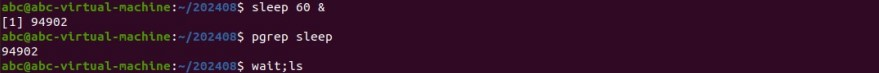
\includegraphics[width=1\textwidth]{002.jpg}
		
\includegraphics[width=1\textwidth]{003.jpg}
	\end{figure}
	
	但是,如果我们在不同的 bash 会话中进行操作,则上述方法就不起作用了。因为 wait 只能对子进程起作用。之前我们没有提过的一个特性是,kill 命令成功退出时其状态码为 0 ,其他状态则是非 0。kill -0 则不会发送信号,但是会在进程不存在时返回一个不为 0 的状态码。请编写一个 bash 函数 pidwait ,它接受一个 pid 作为输入参数,然后一直等待直到该进程结束。您需要使用 sleep 来避免浪费 CPU 性能。
	
	\begin{figure}[H]
		\centering
		
\includegraphics[width=1\textwidth]{004.jpg}
		
\includegraphics[width=1\textwidth]{005.jpg}
	\end{figure}
	
	\subsubsection{题目三}
	创建一个 dc 别名,它的功能是当我们错误的将 cd 输入为 dc 时也能正确执行。
	
	\begin{figure}[H]
		\centering
		
\includegraphics[width=1\textwidth]{005.jpg}
	\end{figure}
	
	\subsubsection{题目四}
	执行 history | awk '\{\$1="";print substr(\$0,2)\}' | sort | uniq -c | sort -n | tail -n 10 来获取您最常用的十条命令,尝试为它们创建别名。
	
	\begin{figure}[H]
		\centering
		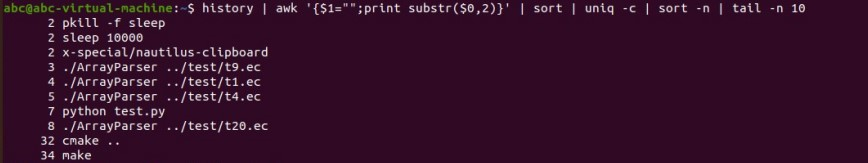
\includegraphics[width=1\textwidth]{006.jpg}
		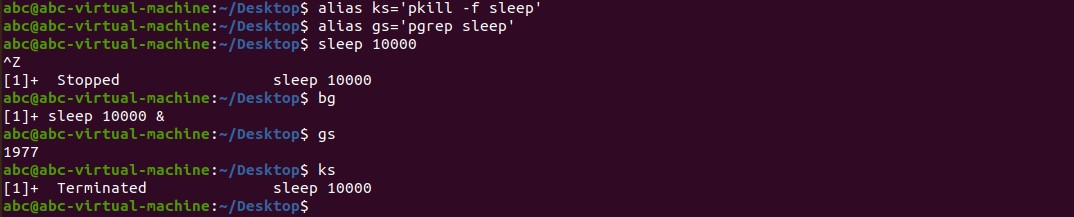
\includegraphics[width=1\textwidth]{008.jpg}
	\end{figure}
	
	\subsection{20个实例}
	
	\paragraph{(1)安装并启动tumx会话:}
	运行 sudo apt-get install tmux 在终端安装tumx
	
	输入 tmux 创建一个新的 tmux 会话
	
	\begin{figure}[H]
		\centering
		
\includegraphics[width=1\textwidth]{011.jpg}
		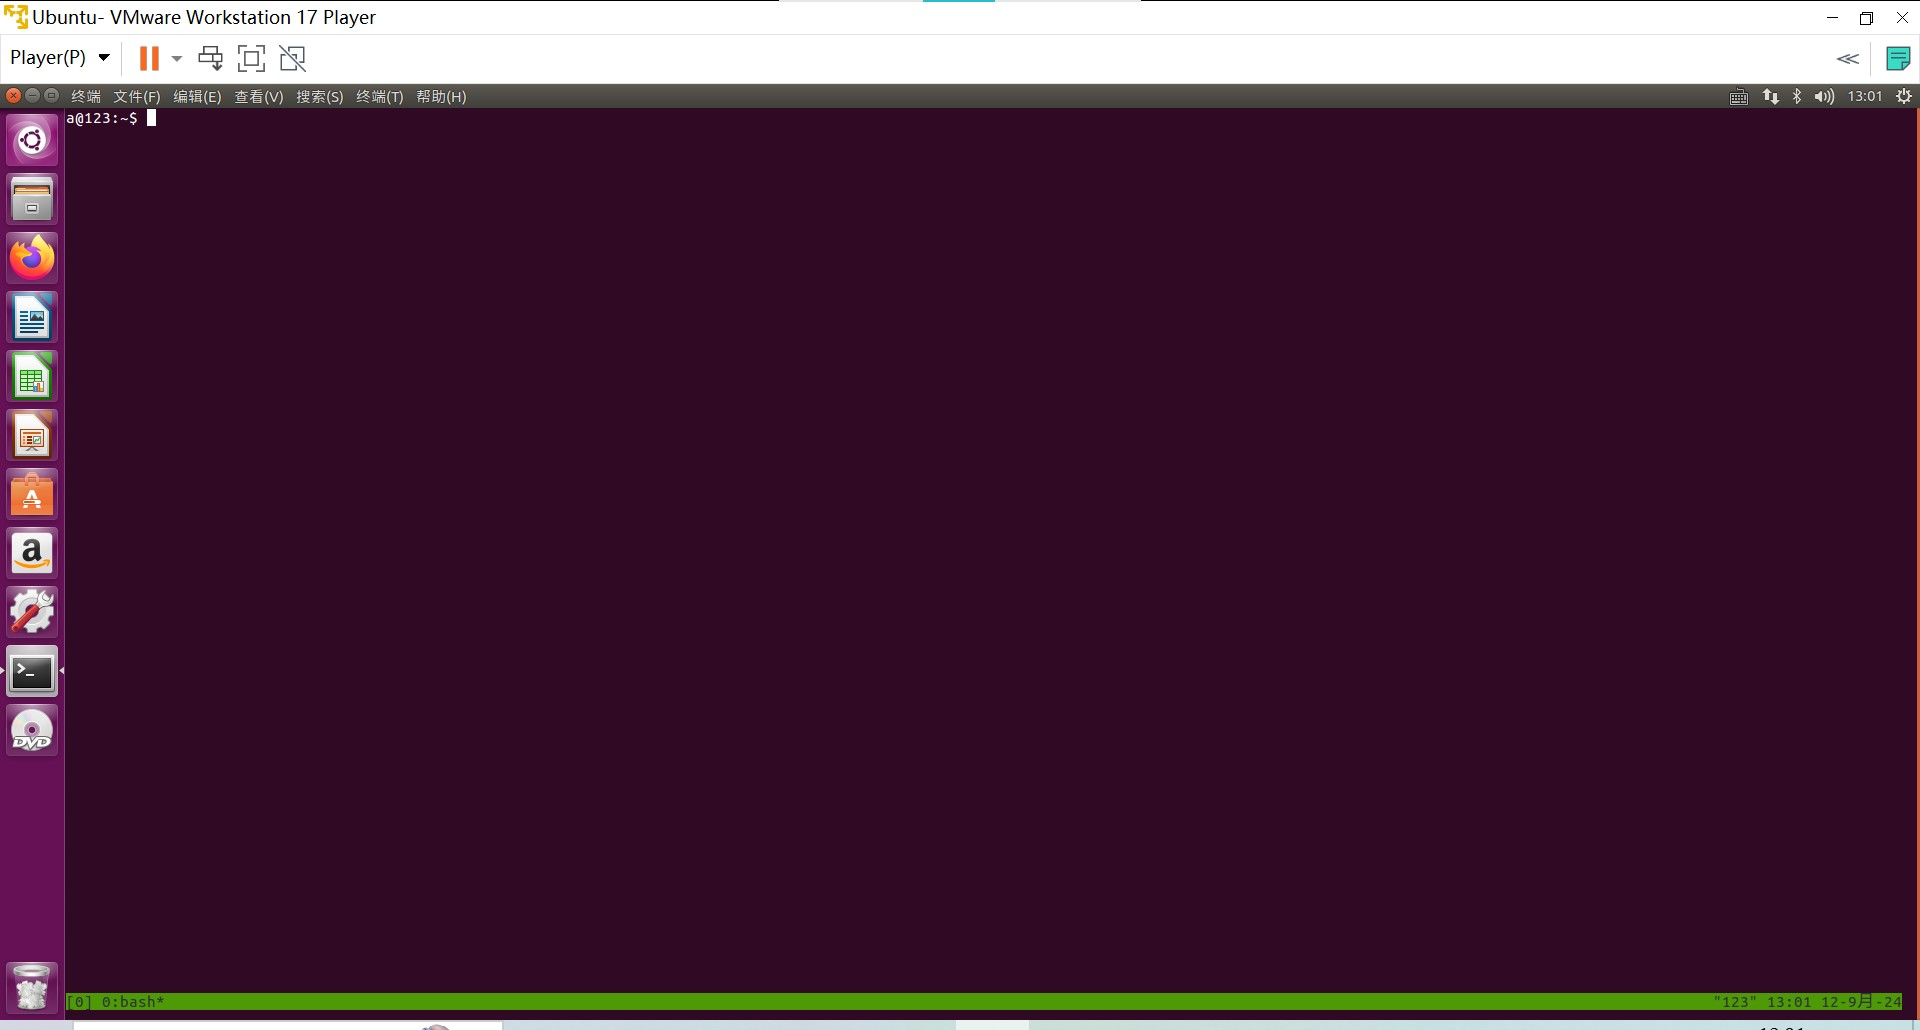
\includegraphics[width=1\textwidth]{010.jpg}
	\end{figure}
	
	\paragraph{(2)显示帮助:}	
	按下组合键ctrl+b ?
	
	\begin{figure}[H]
		\centering
		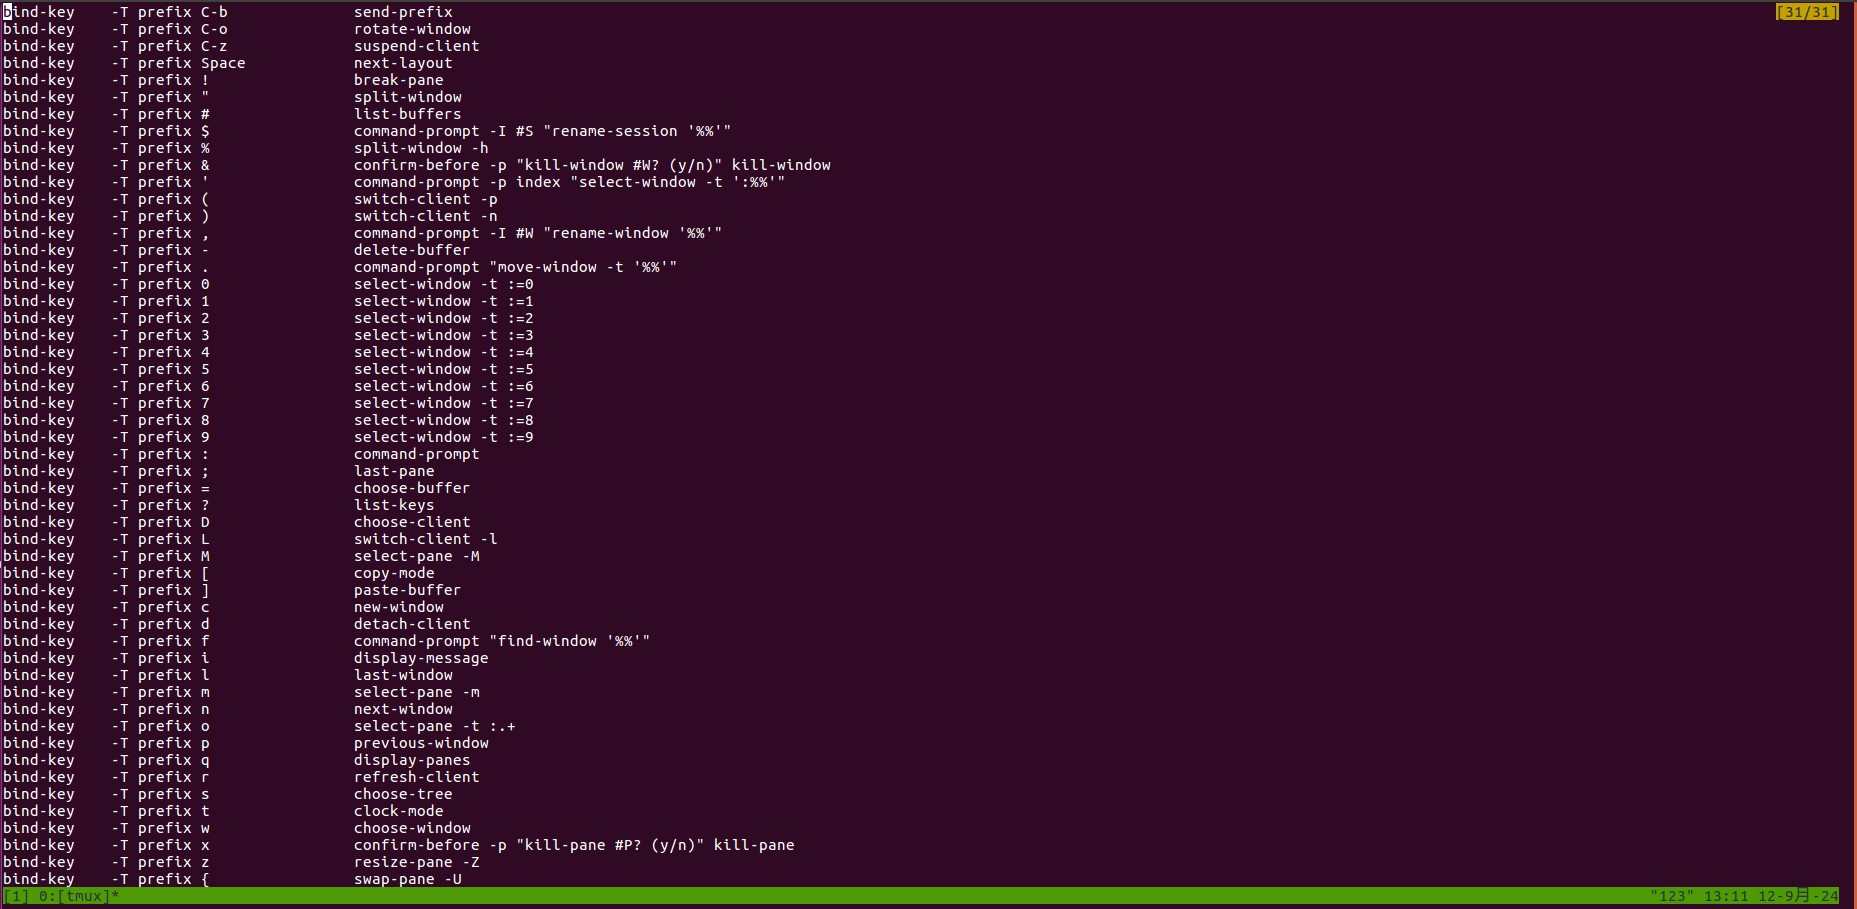
\includegraphics[width=1\textwidth]{012.jpg}
	\end{figure}
	
	\paragraph{(3)退出当前tmux会话:}
	按下组合键ctrl+d 或者显式输入exit命令
	
	\begin{figure}[H]
		\centering
		
\includegraphics[width=1\textwidth]{013.jpg}
	\end{figure}
	
	\paragraph{(4)tmux new -s <session-name>:}
	上面命令新建一个指定名称的会话。	
	
	\begin{figure}[H]
		\centering
		
\includegraphics[width=1\textwidth]{014.jpg}
		
\includegraphics[width=1\textwidth]{015.jpg}
	\end{figure}
	
	
	\paragraph{(5)将窗格拆分为两个窗格:}	
	按下组合键ctrl+b \% 将窗格拆分为左窗格和右窗格。
	
	按下组合键ctrl+b " 将窗格拆分为顶部窗格和底部窗格。
	
	要切换到不同窗格,可按下ctrl+b 方向键进行切换。
	
	\begin{figure}[H]
		\centering
		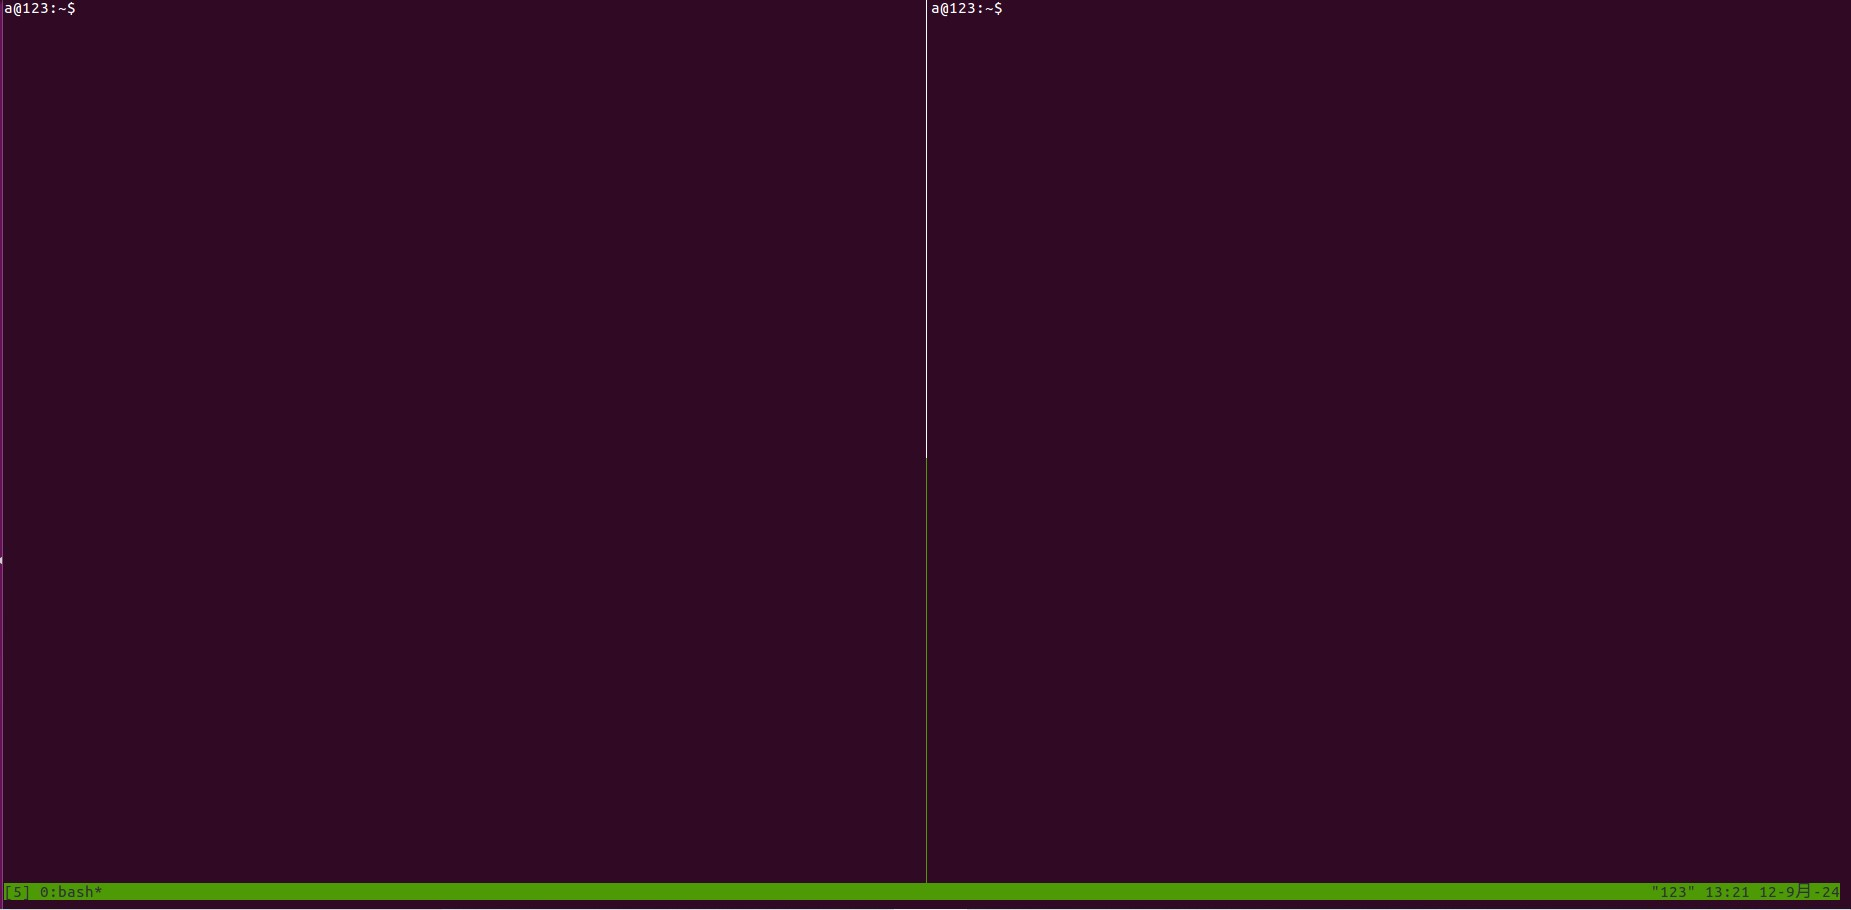
\includegraphics[width=1\textwidth]{016.jpg}
		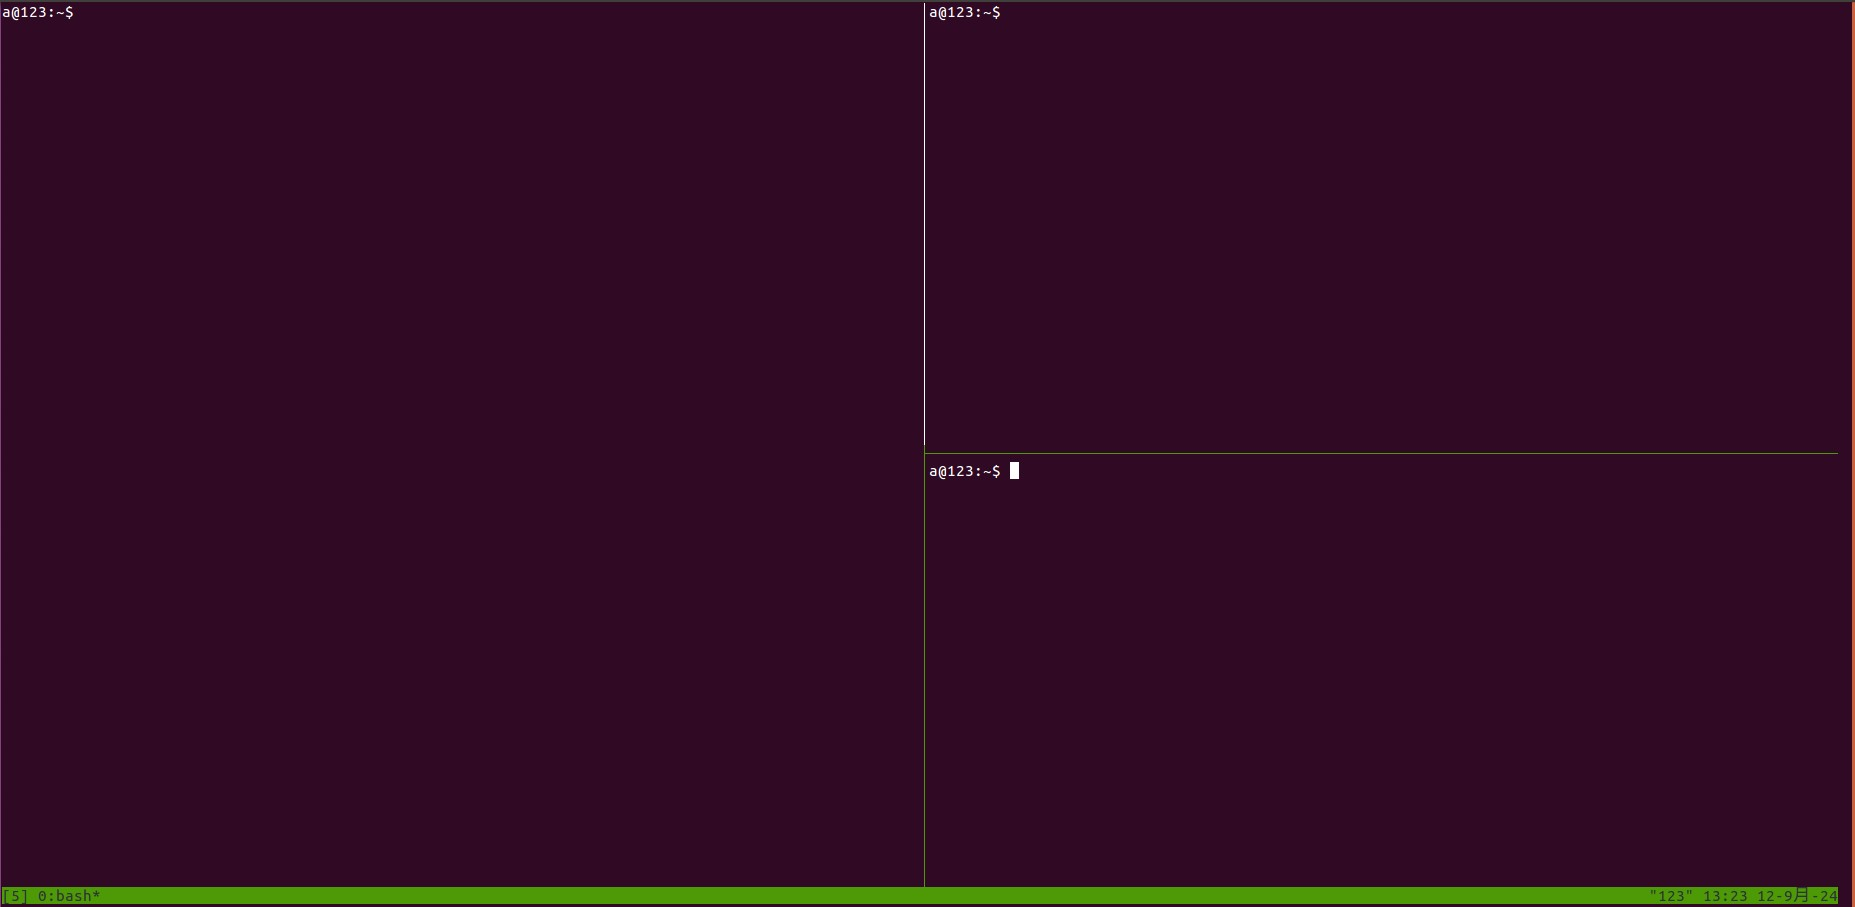
\includegraphics[width=1\textwidth]{017.jpg}
	\end{figure}
	
	\paragraph{(6)分离对话:}	
	按下组合键Ctrl+b d 或者 输入tmux detach命令,就会将当前会话与窗口分离。
	这样会退出当前 Tmux 窗口,但是会话和里面的进程仍然在后台运行。
	
	\begin{figure}[H]
		\centering
		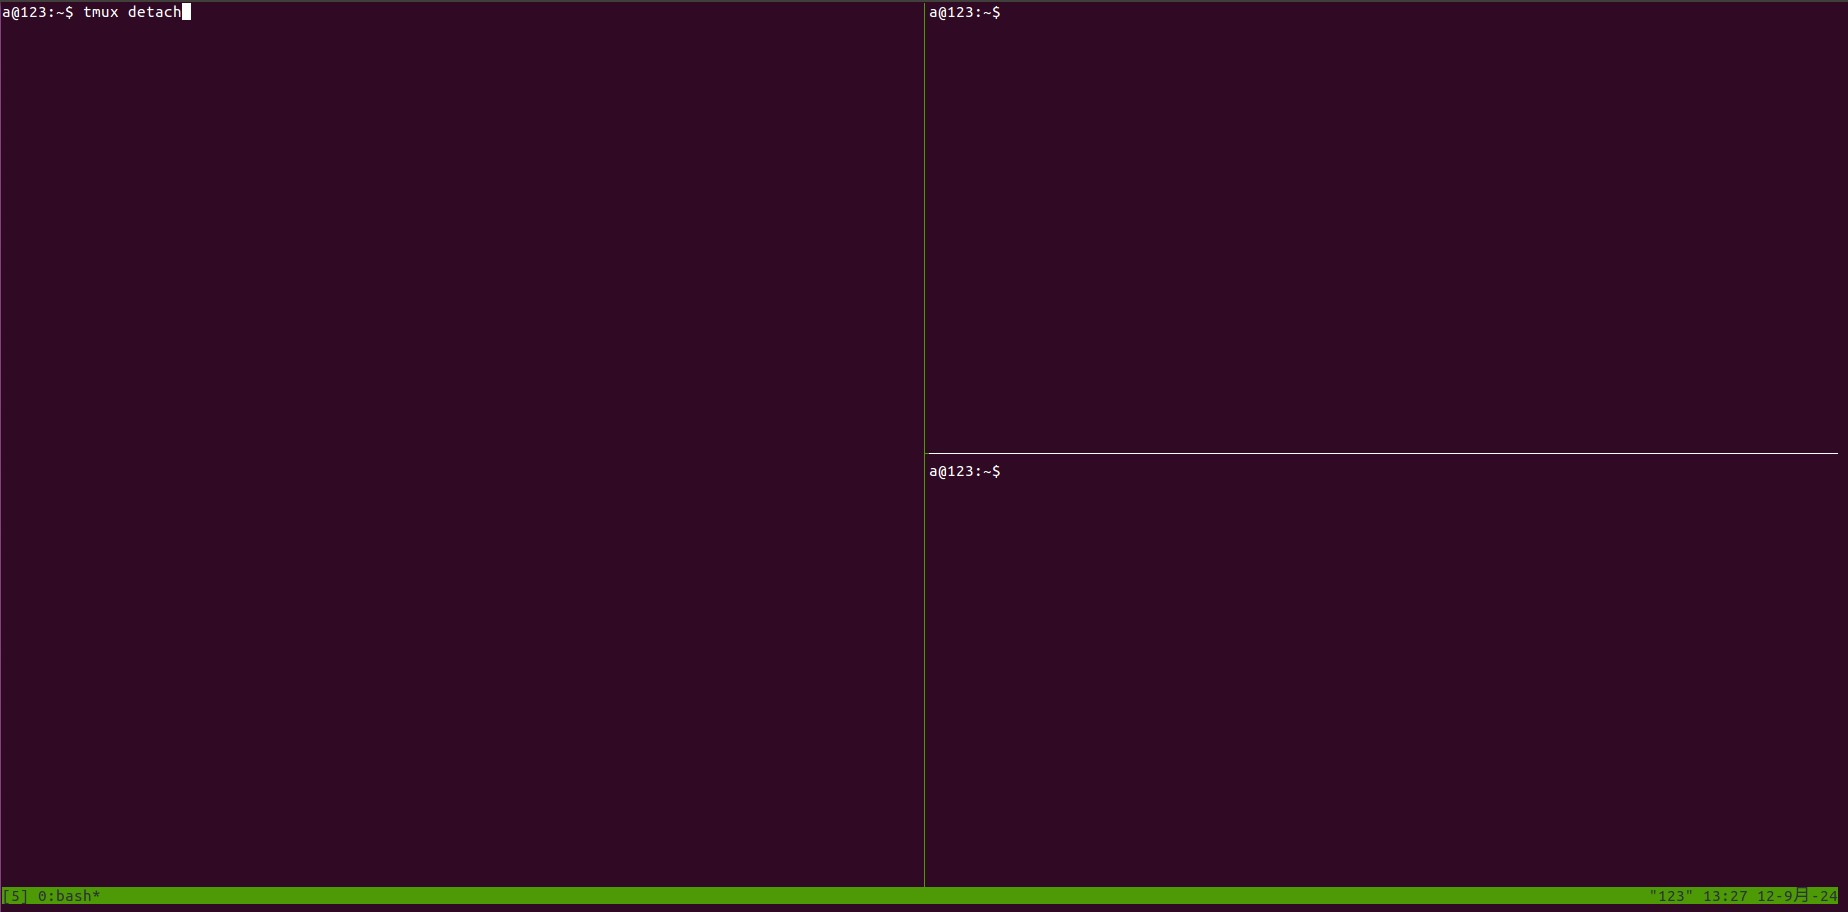
\includegraphics[width=1\textwidth]{018.jpg}
		
\includegraphics[width=1\textwidth]{019.jpg}
	\end{figure}
	
	\paragraph{(7)tmux ls:}
	查看当前所有的 Tmux 会话。
	
	\begin{figure}[H]
		\centering
		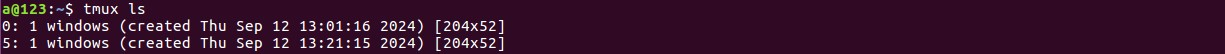
\includegraphics[width=1\textwidth]{020.jpg}
	\end{figure}
	
	\paragraph{(8)tmux attach:}
	重新接入某个已存在的会话。	
	
	\begin{figure}[H]
		\centering
		
\includegraphics[width=1\textwidth]{021.jpg}
		
\includegraphics[width=1\textwidth]{022.jpg}
	\end{figure}
	
	\paragraph{(9)tmux kill-session:}
	杀死某个会话。	
	
	\begin{figure}[H]
		\centering
		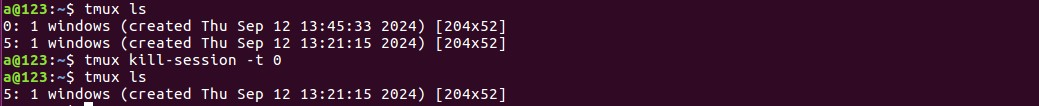
\includegraphics[width=1\textwidth]{023.jpg}
	\end{figure}
	
	\paragraph{(10)tmux switch:}
	切换会话。	
	
	\begin{figure}[H]
		\centering
		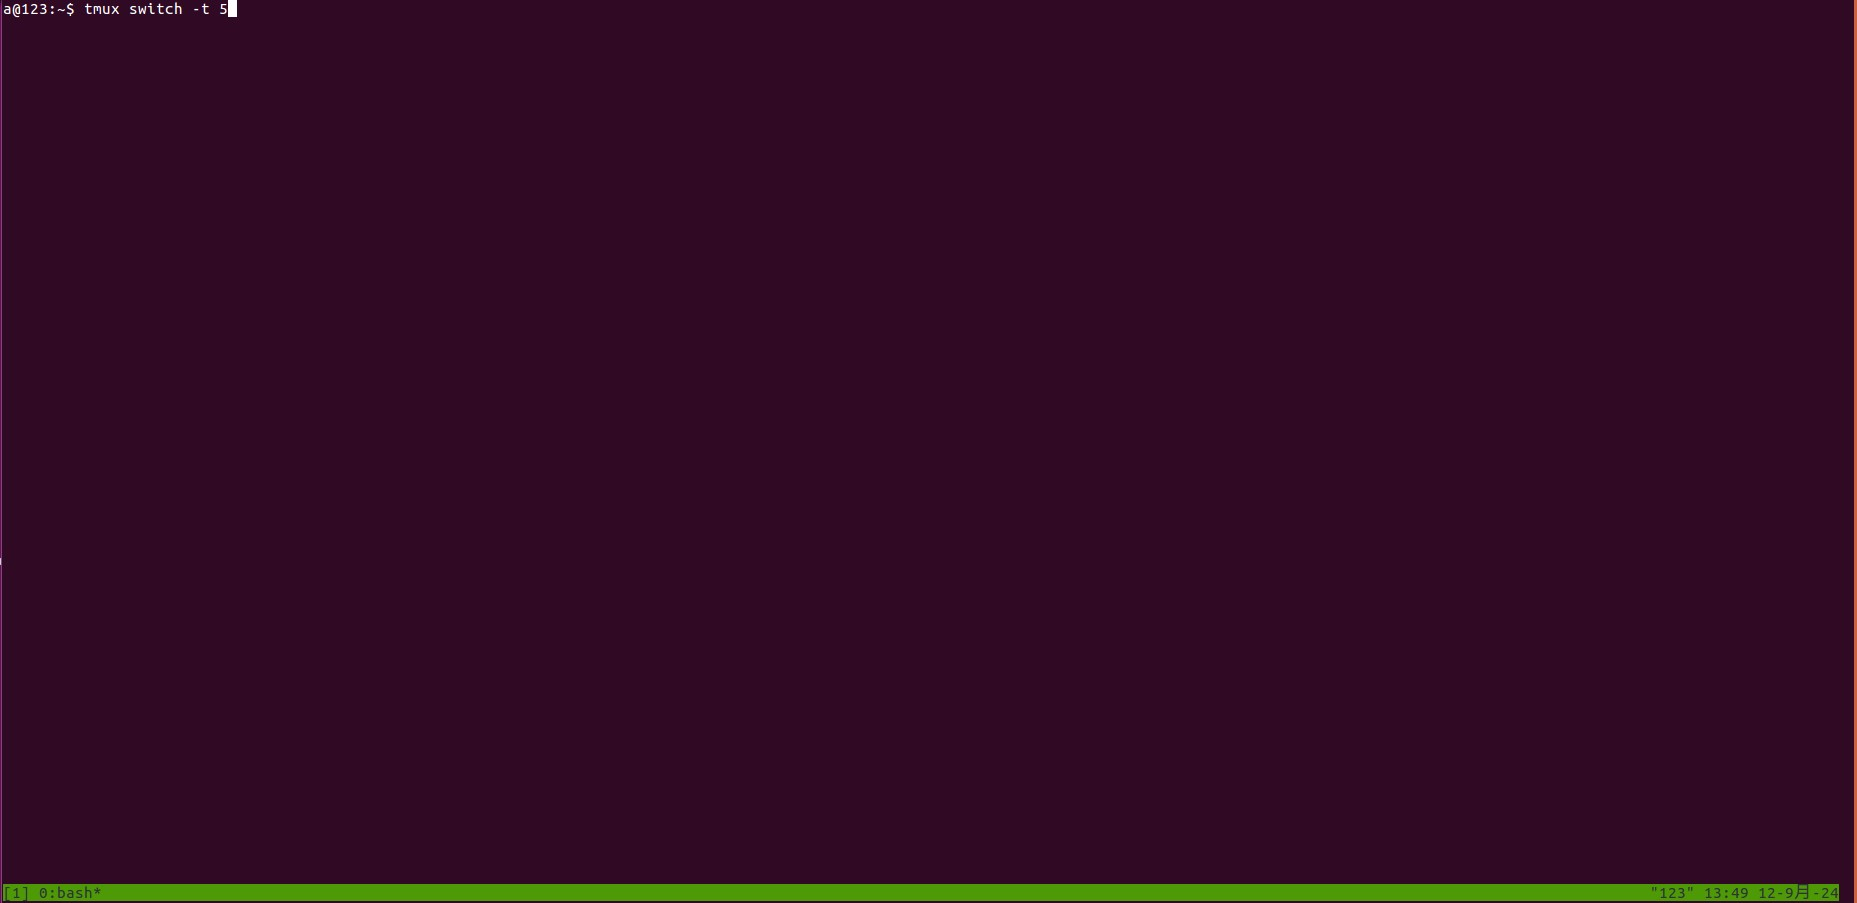
\includegraphics[width=1\textwidth]{024.jpg}
		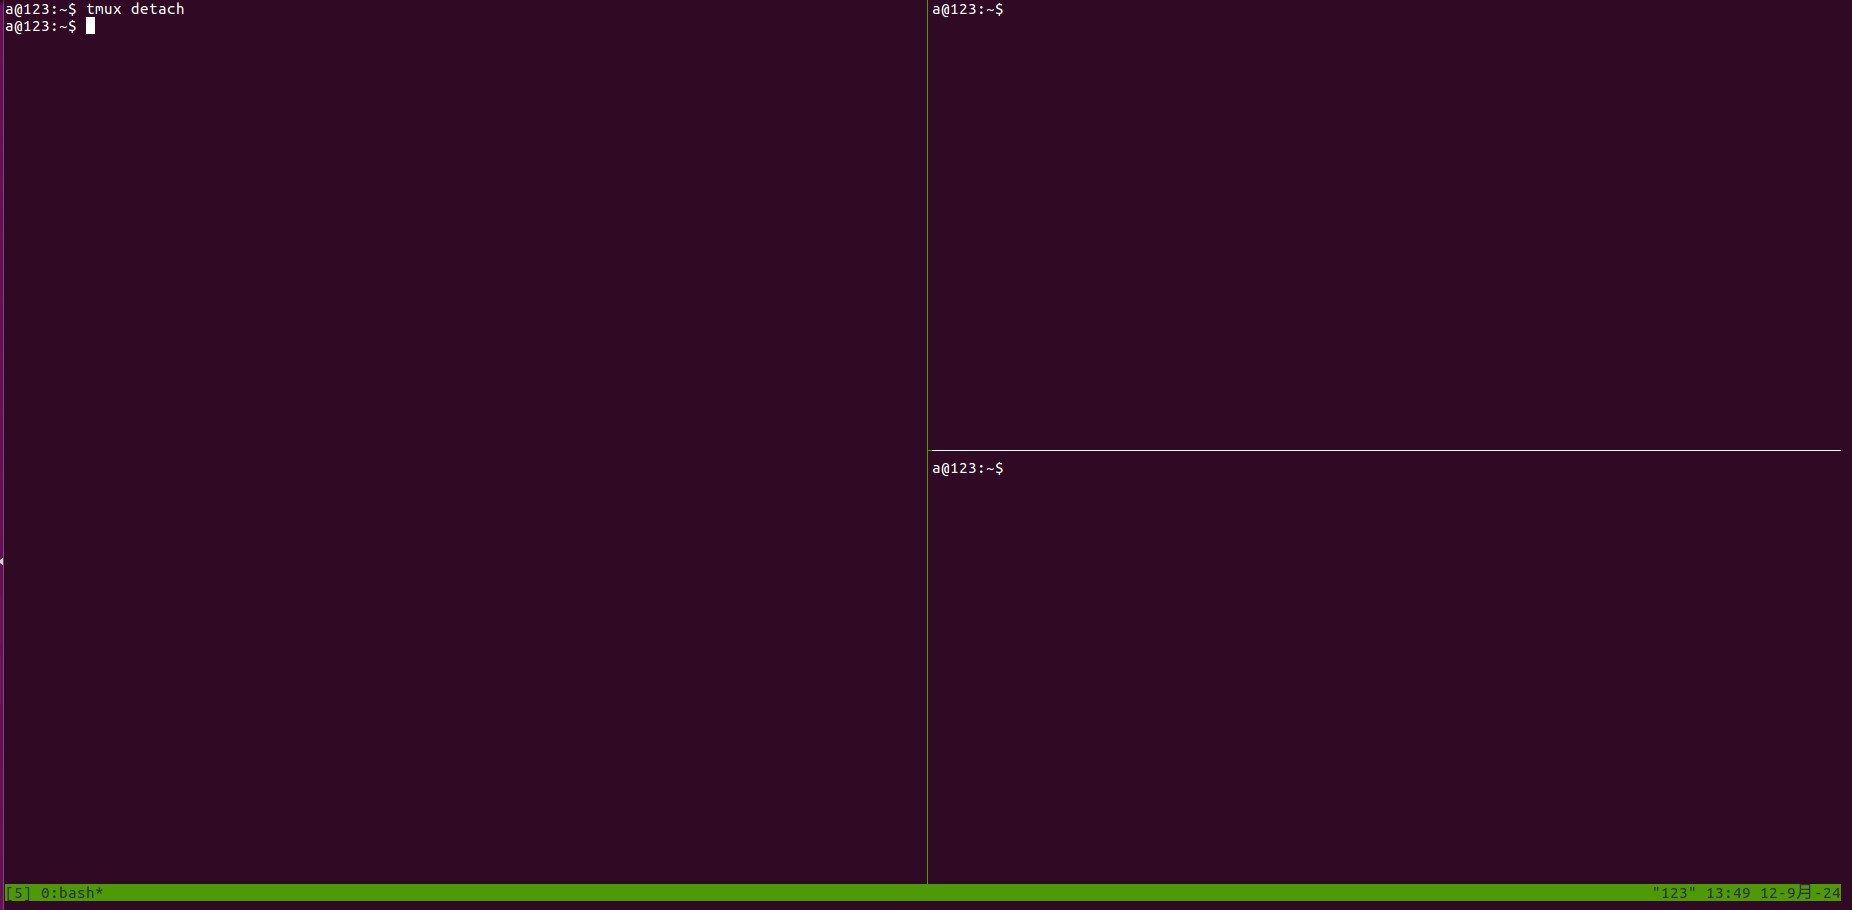
\includegraphics[width=1\textwidth]{025.jpg}
	\end{figure}
	
	\paragraph{(11)tmux rename-session:}
	重命名会话。	
	
	\begin{figure}[H]
		\centering
		
\includegraphics[width=1\textwidth]{026.jpg}
	\end{figure}
	
	\paragraph{(12)创建ssh密钥对:}
	输入命令 ssh-keygen -o -a 100 -t ed25519
	
	\begin{figure}[H]
		\centering
		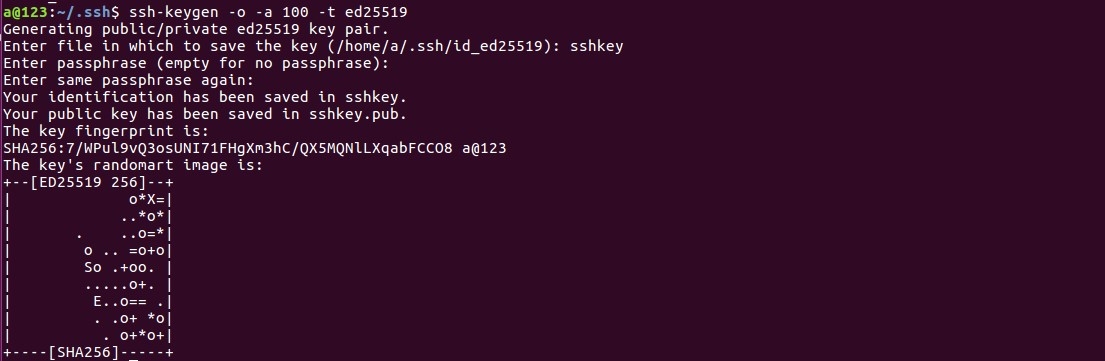
\includegraphics[width=1\textwidth]{027.jpg}
	\end{figure}
	
	\paragraph{(13)ssh远程连接:}	
	输入命令 ssh <username>@<ip> [-p <port>]
	
	\begin{figure}[H]
		\centering
		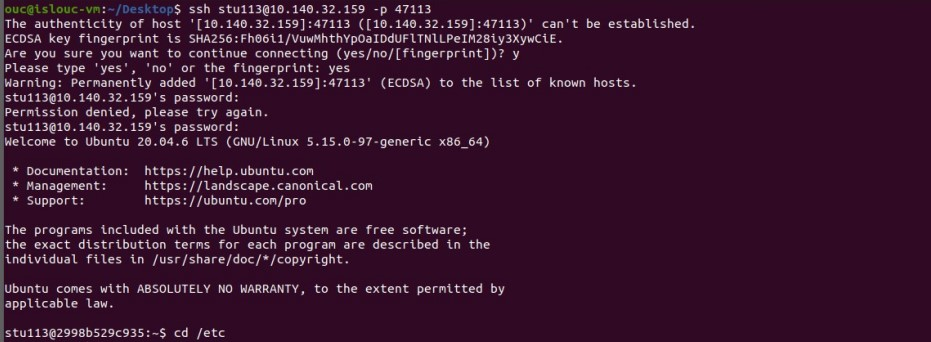
\includegraphics[width=1\textwidth]{028.jpg}
	\end{figure}
	
	\paragraph{(14)python入门:}安装并配置pycharm,在pycharm上创建一个python项目,写示例输出helloworld。
	
	\begin{figure}[H]
		\centering
		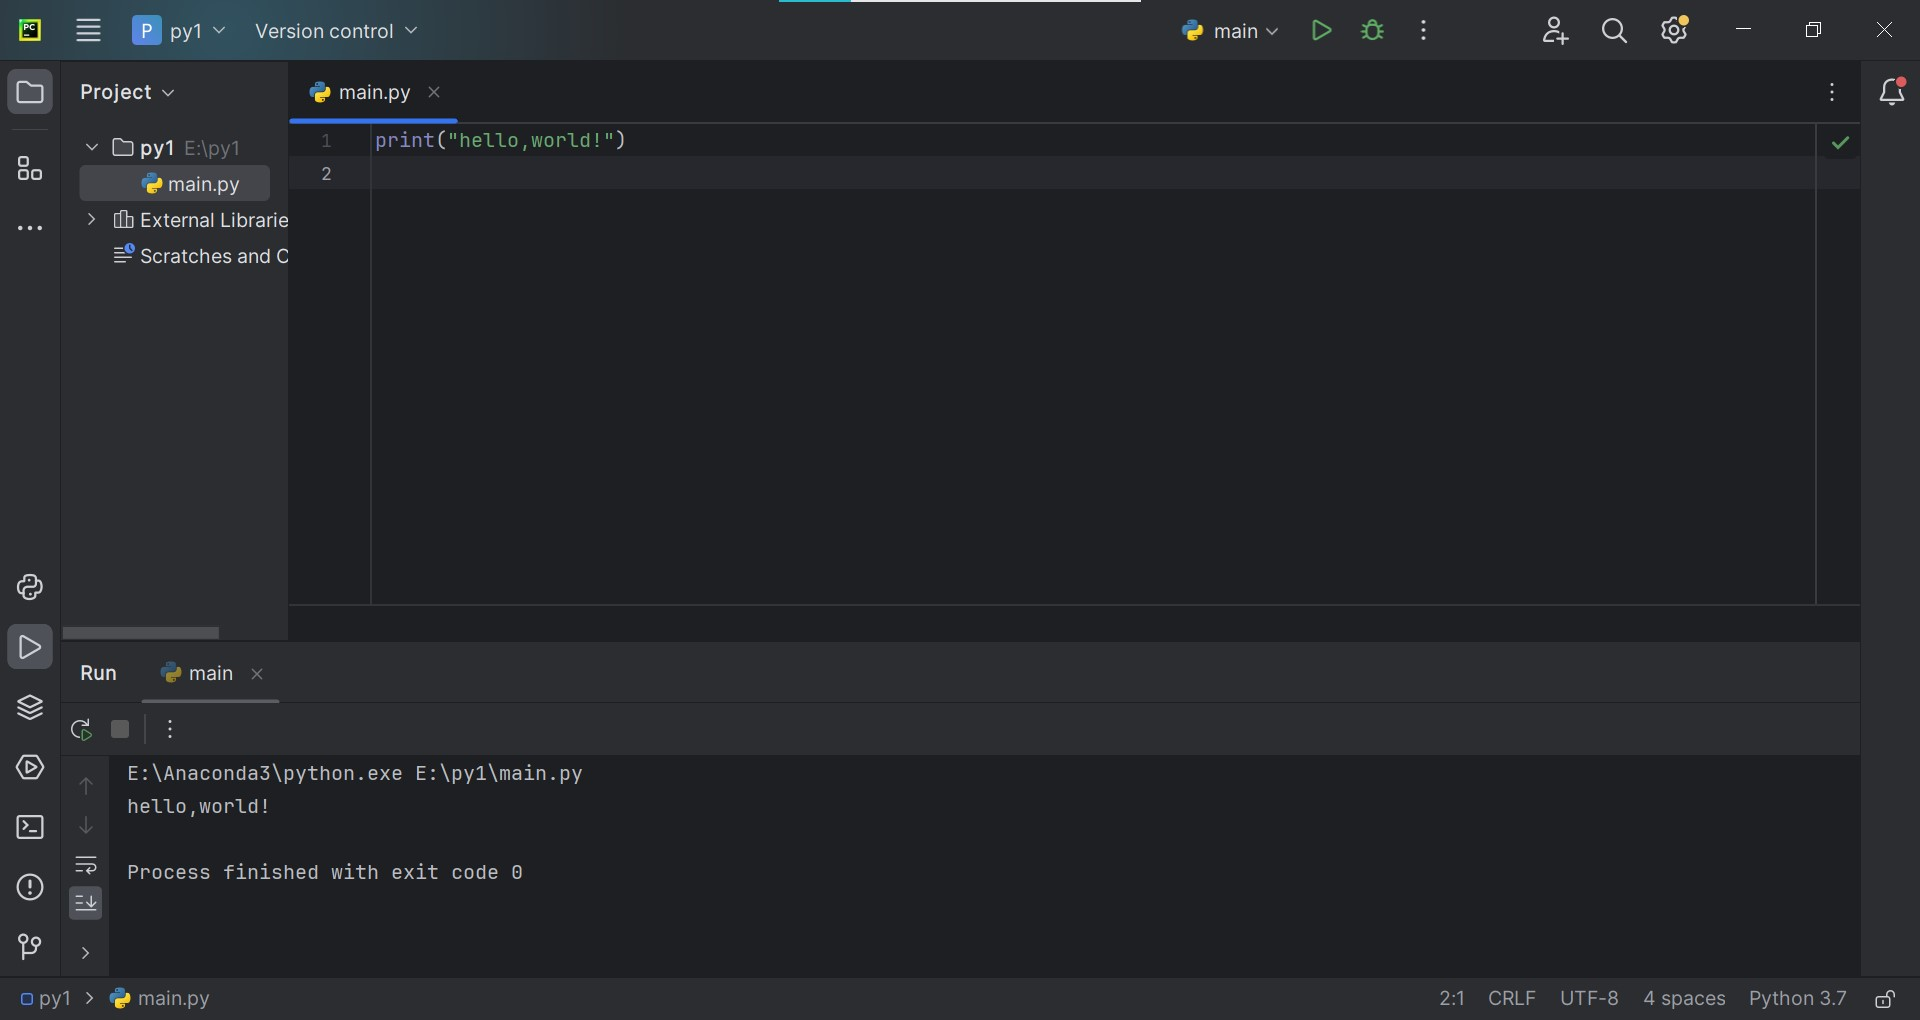
\includegraphics[width=1\textwidth]{029.jpg}
	\end{figure}
	
	\paragraph{(15)python命令行参数:}
	在终端命令行使用-h参数查看各参数帮助信息。
	
	\begin{figure}[H]
		\centering
		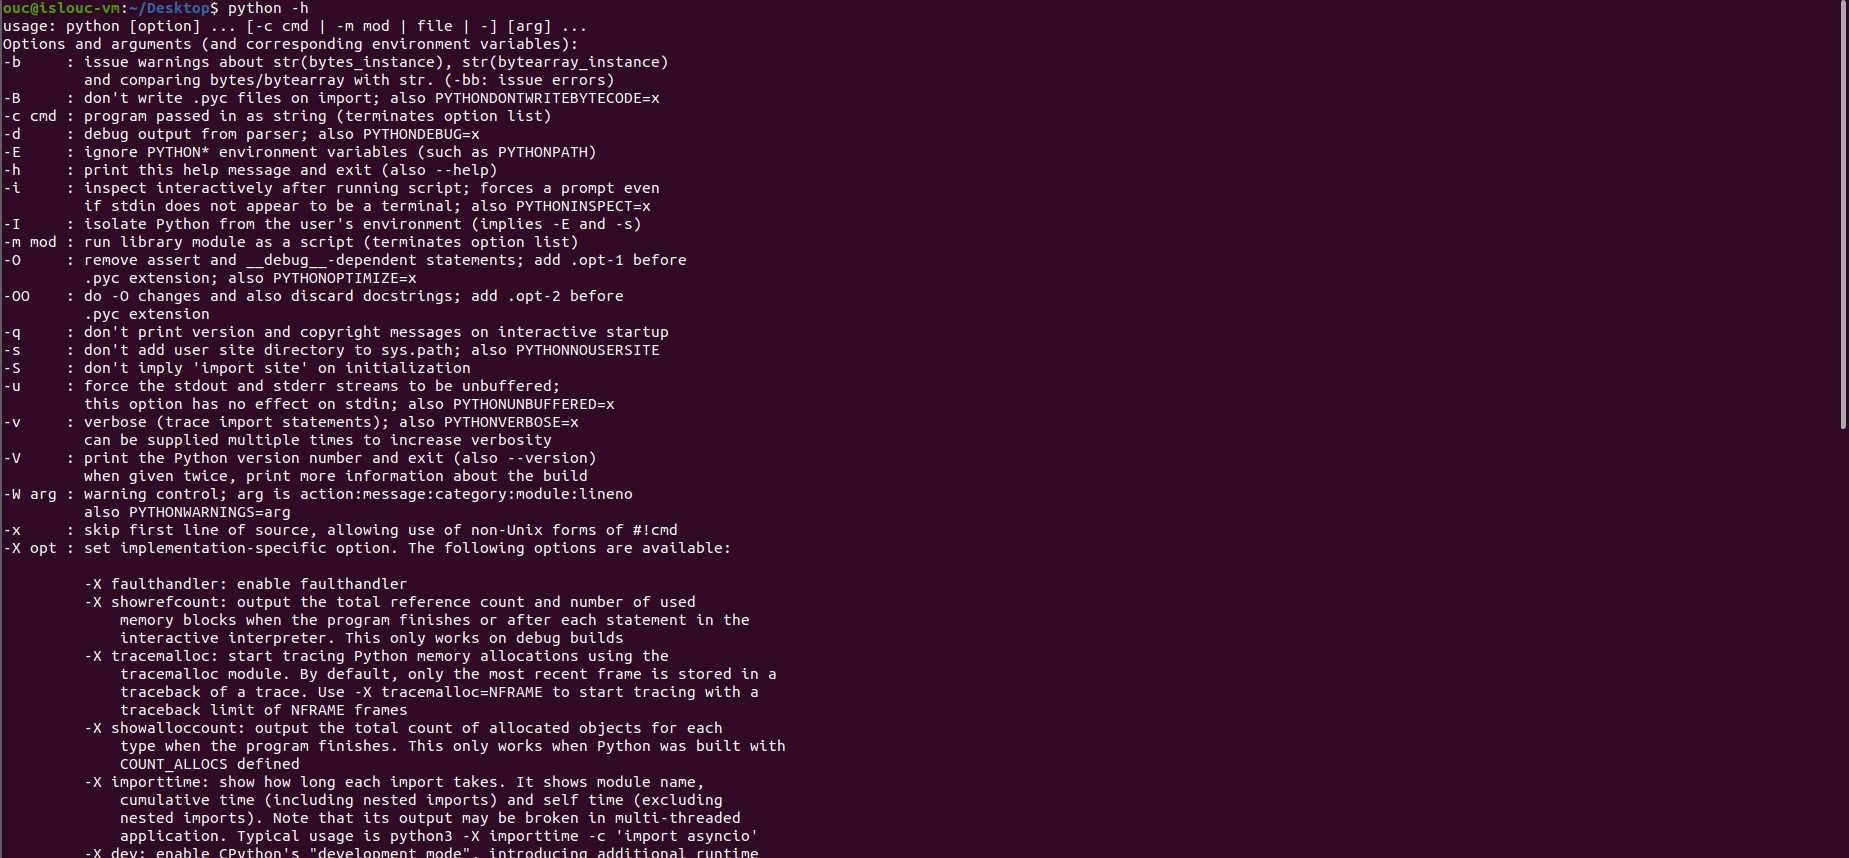
\includegraphics[width=1\textwidth]{030.jpg}
	\end{figure}
	
	\paragraph{(16)python实例-素数判断:}	
	在虚拟机终端环境编写python程序实现素数判断的功能。
	
	(代码已上传至github库-task2-py2.py)
	
	\begin{figure}[H]
		\centering
		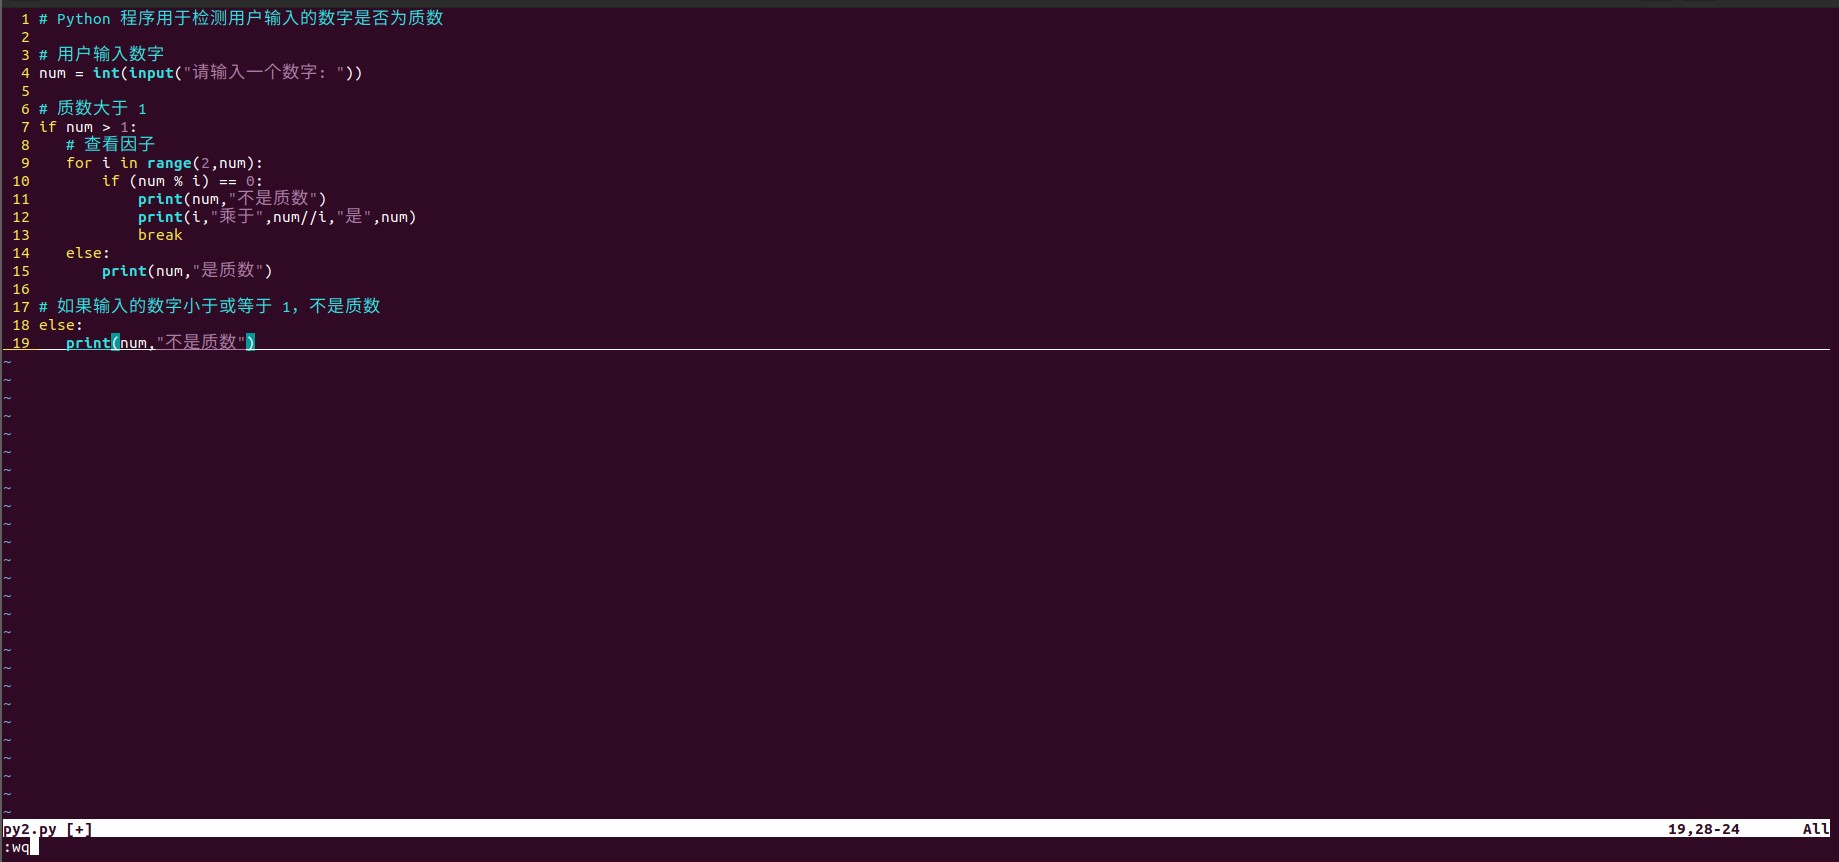
\includegraphics[width=1\textwidth]{031.jpg}
		
\includegraphics[width=1\textwidth]{032.jpg}
	\end{figure}
	
	\paragraph{(17)python视觉-图像基本操作:}
	在pycharm写Python程序,引用PIL库,实现修改图片大小、转换灰度图像,另存为其他图像格式的功能。
	
	(具体代码及输出结果已上传至github库-task2-py3)
	
	\begin{figure}[H]
		\centering
		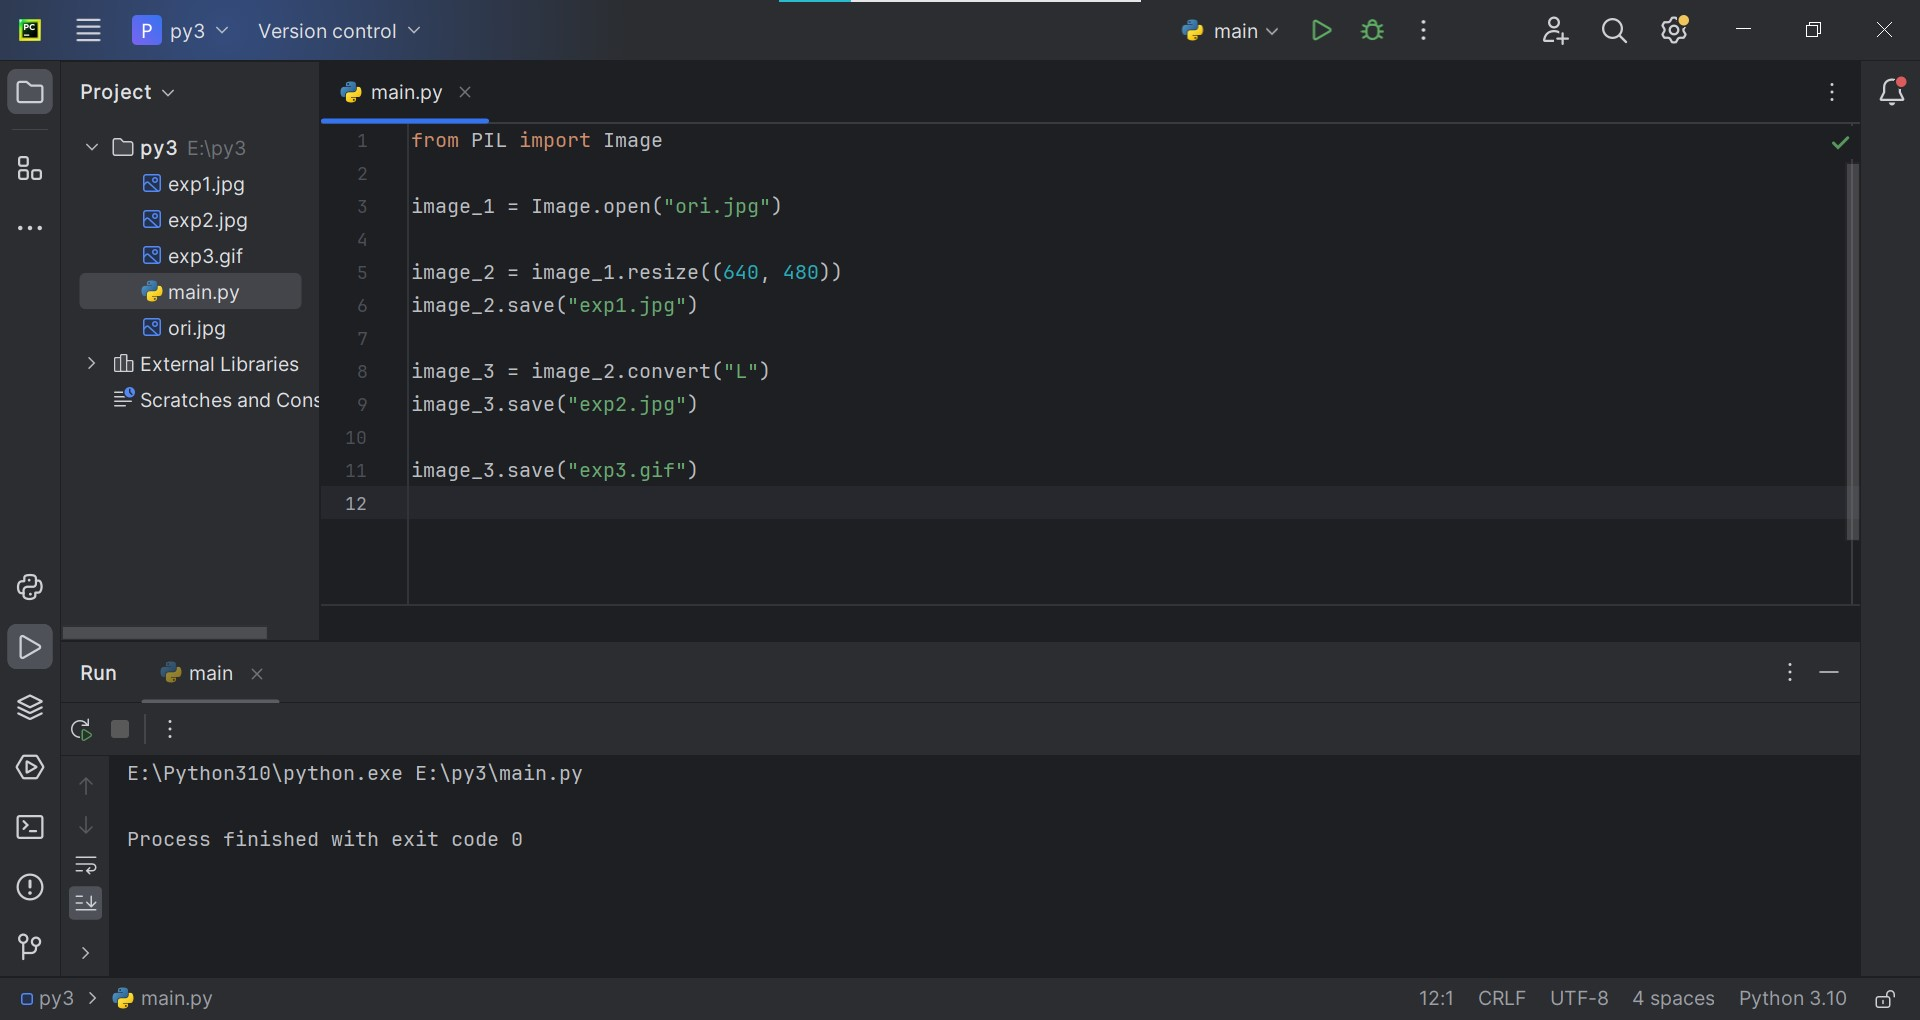
\includegraphics[width=1\textwidth]{033.jpg}
		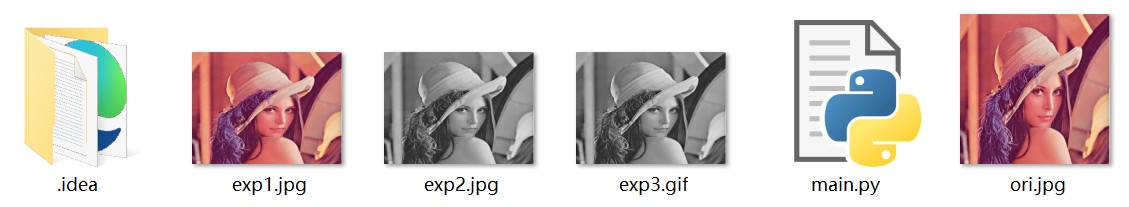
\includegraphics[width=1\textwidth]{034.jpg}
	\end{figure}
	
	\paragraph{(18)python视觉-频率域图像操作:}	
	在pycharm写Python程序对图片进行傅立叶变换、DCT变换并查看频谱图。
	
	\paragraph{实例要求:}
	用Python写程序,对目录下的图像(1.bmp,2.bmp,2.jpg,3.bmp,4.bmp),实现: 
	
	(1)查看不同图像的傅立叶变换的图像 查看不同图像的DCT(离散余弦)变换。 
	
	(2)对变换后得到的频谱图使用空间域图像增强的方法增强效果。
	
	(3)采用低通滤波器和高通滤波器对图像进行频率域滤波,设置不同的阈值,查看效果。
	
	\paragraph{实例解答:}
	分如下四步:
	
	(1)读取图像列表(1.bmp,2.bmp,2.jpg,3.bmp,4.bmp)。
	
	(2)对于列表中每一个图像,用numpy库的np.fft.fft2()和np.fft.fftshift()函数对图像进行快速傅里叶变换,保存图像;用opencv库的cv2.dct()函数对图像进行离散余弦变换,保存图像。
	
	(3)对上一步得到的频谱图使用空间域图像增强的方法增强效果。修改图像灰度,这里用log对数变换,增强图像较暗区域的细节,使频谱图可视化。保存结果。
	
	(4)分别采用低通滤波器和高通滤波器对图像进行频率域滤波。首先通过dft()和fftshift()函数对图像进行傅里叶变换,再设置掩膜mask,将掩膜与傅里叶变化后的图像相乘,保留低频部分,再进行傅里叶逆变换idft()得到滤波结果。对低通滤波和高通滤波设置不同的掩膜及阈值yuzhi,重复上述操作,保存并查看效果。
	
	(具体代码及输出结果已上传至github库-task2-py4)
	
	\begin{figure}[H]
		\centering
		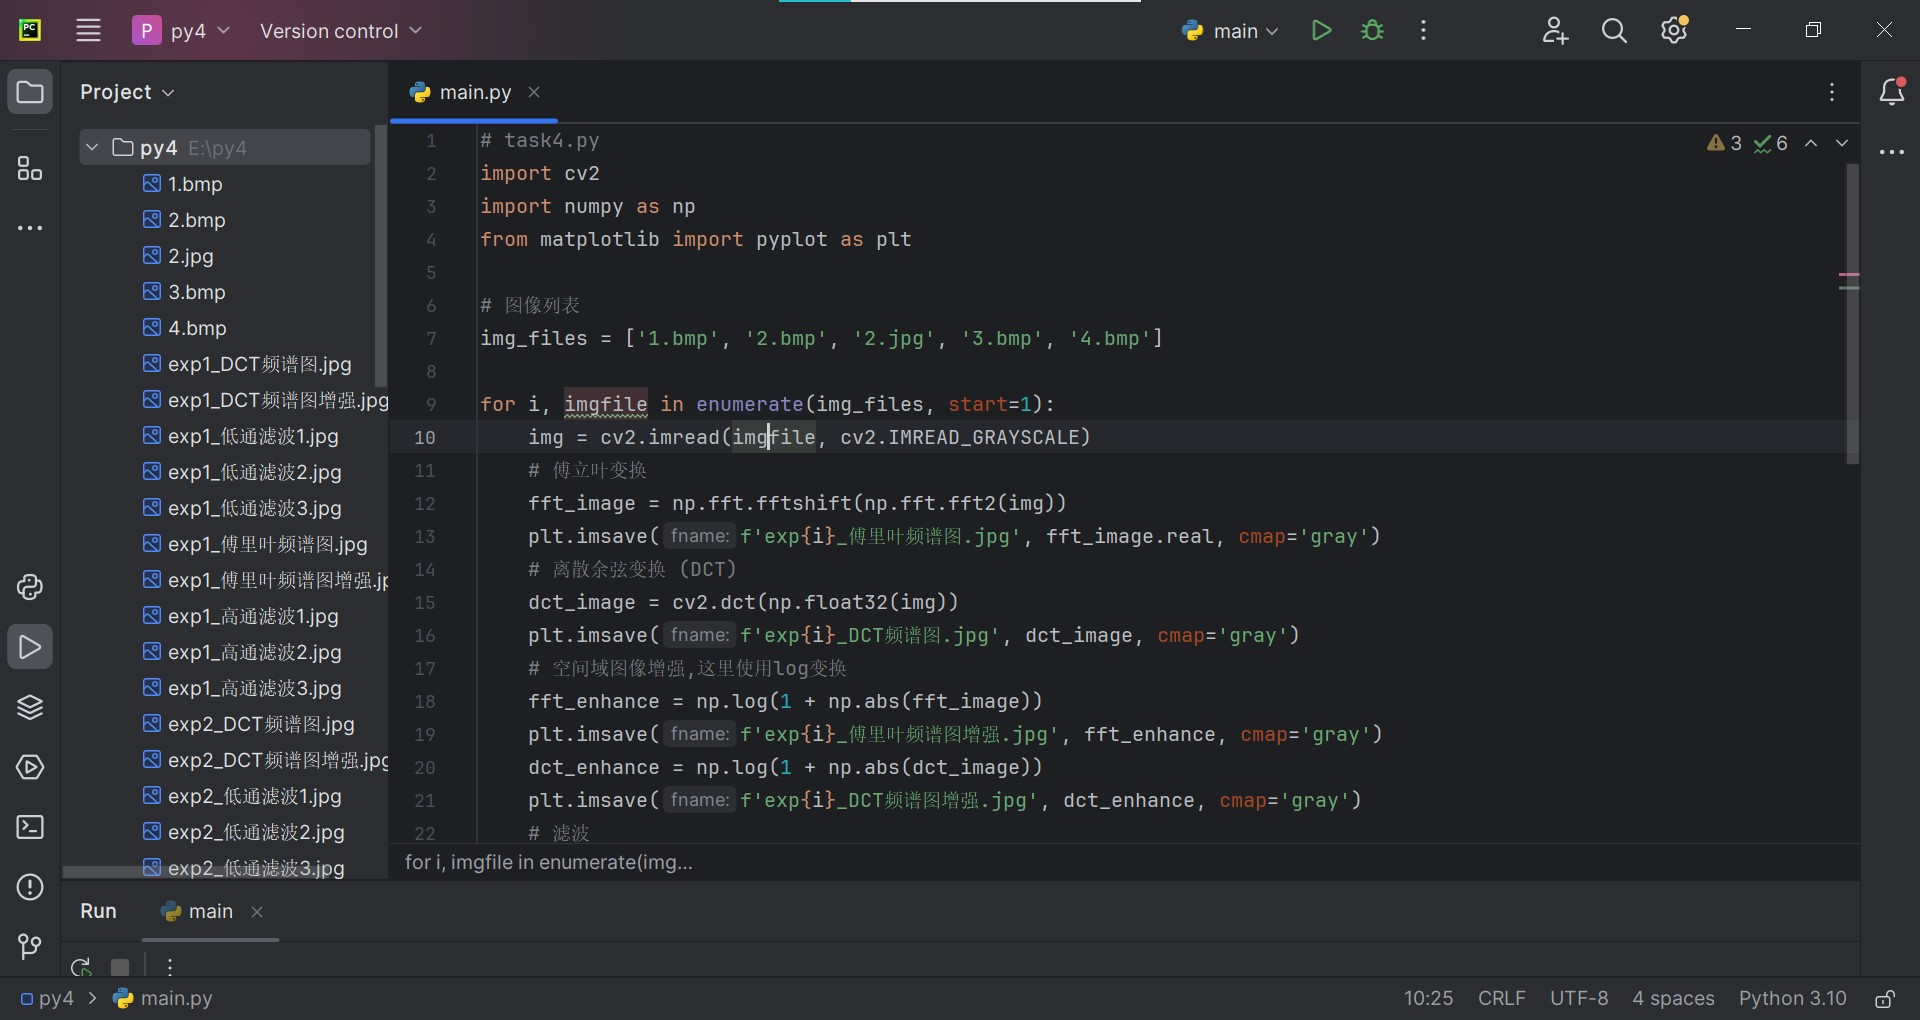
\includegraphics[width=1\textwidth]{035.jpg}
		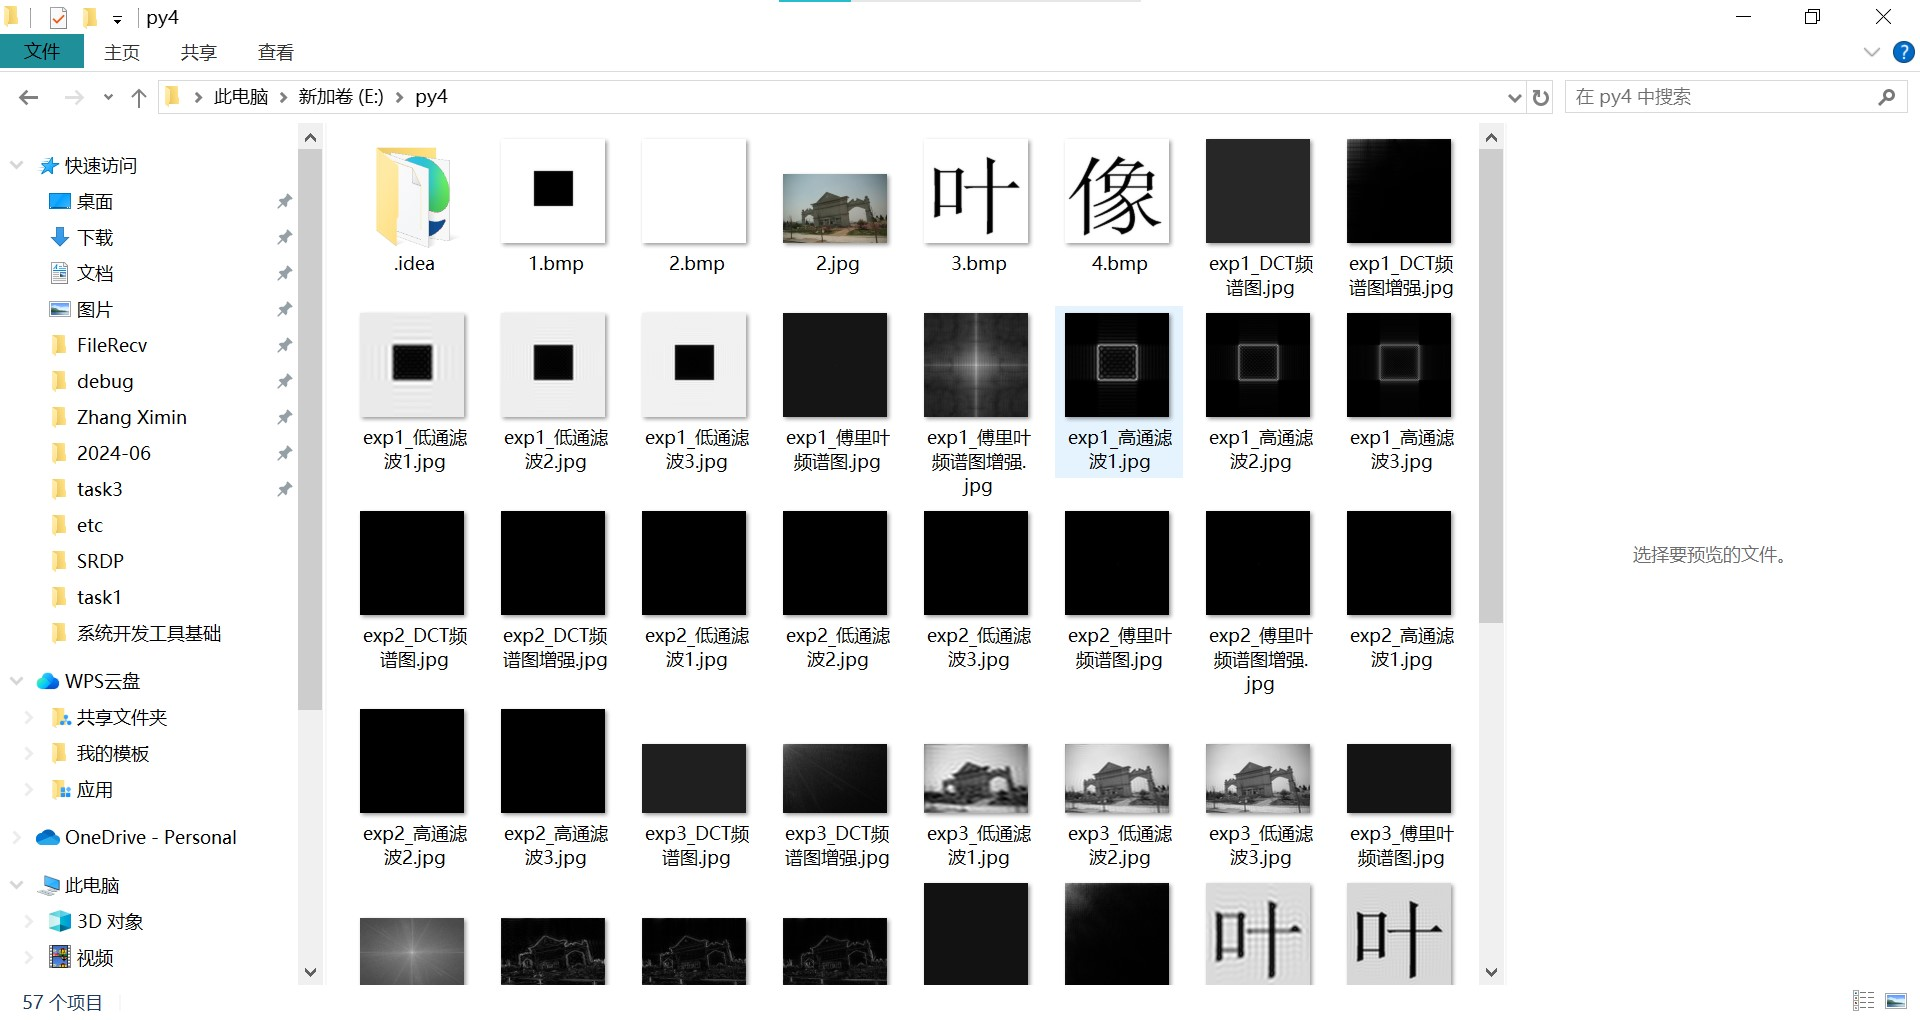
\includegraphics[width=1\textwidth]{036.jpg}
	\end{figure}
	
	\paragraph{(19)python视觉-空间域图像增强}
	在pycharm写Python程序对图片进行直方图查看、高斯滤波磨皮操作。
	
	\paragraph{实例要求:}
	用Python写一段程序,针对提供的图片 ori1.jpg 和 ori2.jpg,实现:
	
	(1)查看ori1.jpg的直方图并保存;对ori1.jpg取反,再查看直方图并保存;对ori1.jpg使用直方图均衡,再查看直方图并保存。
	
	(2)对人脸ori2.jpg进行滤波等操作实现类似美图秀秀的磨皮功能,并对比磨皮前后直方图变化。
	
	\paragraph{实例解答:}
	(1)利用opencv库读取图像并查看直方图,plt库展示并保存直方图。取反图=255-原图,直方图均衡使用cv2.equalizeHist()函数。
	
	(2)磨皮使用cv2.GaussianBlur()进行高斯模糊,plt库展示并保存直方图。

	(具体代码及输出结果已上传至github库-task2-py5)

	\begin{figure}[H]
		\centering
		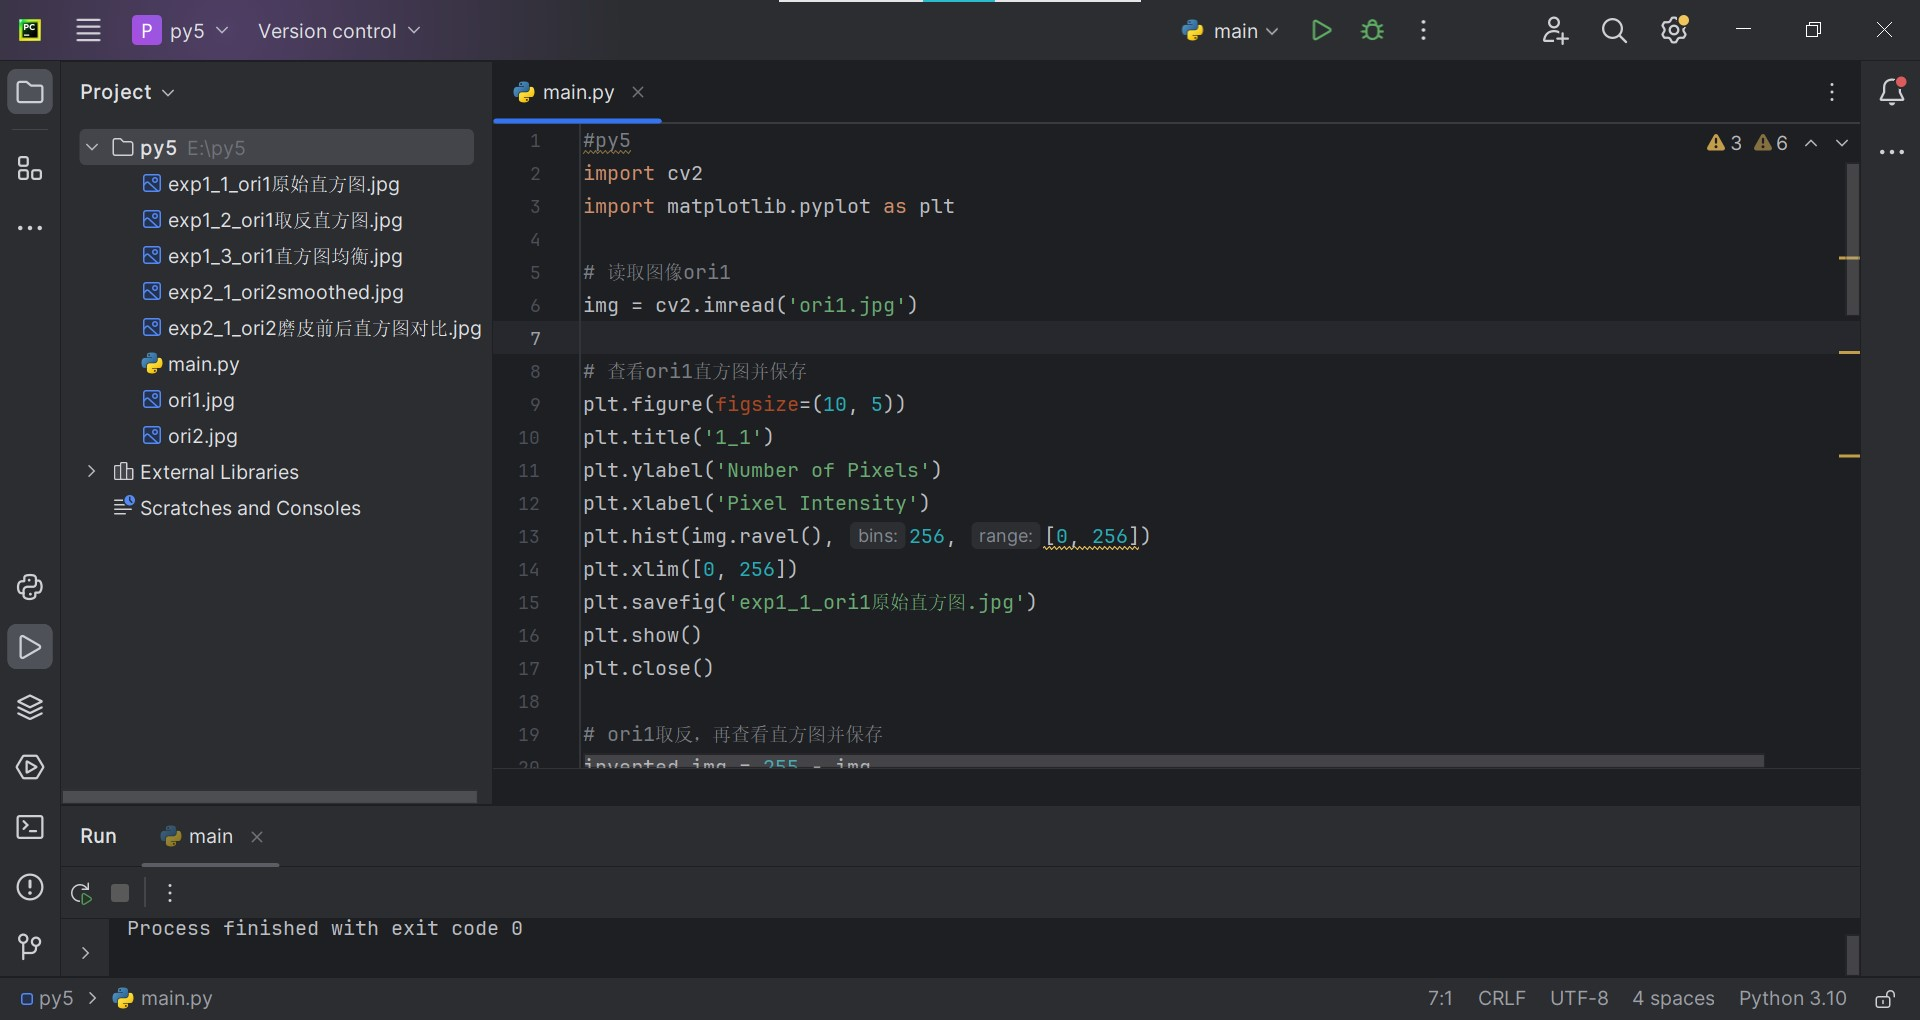
\includegraphics[width=1\textwidth]{037.jpg}
		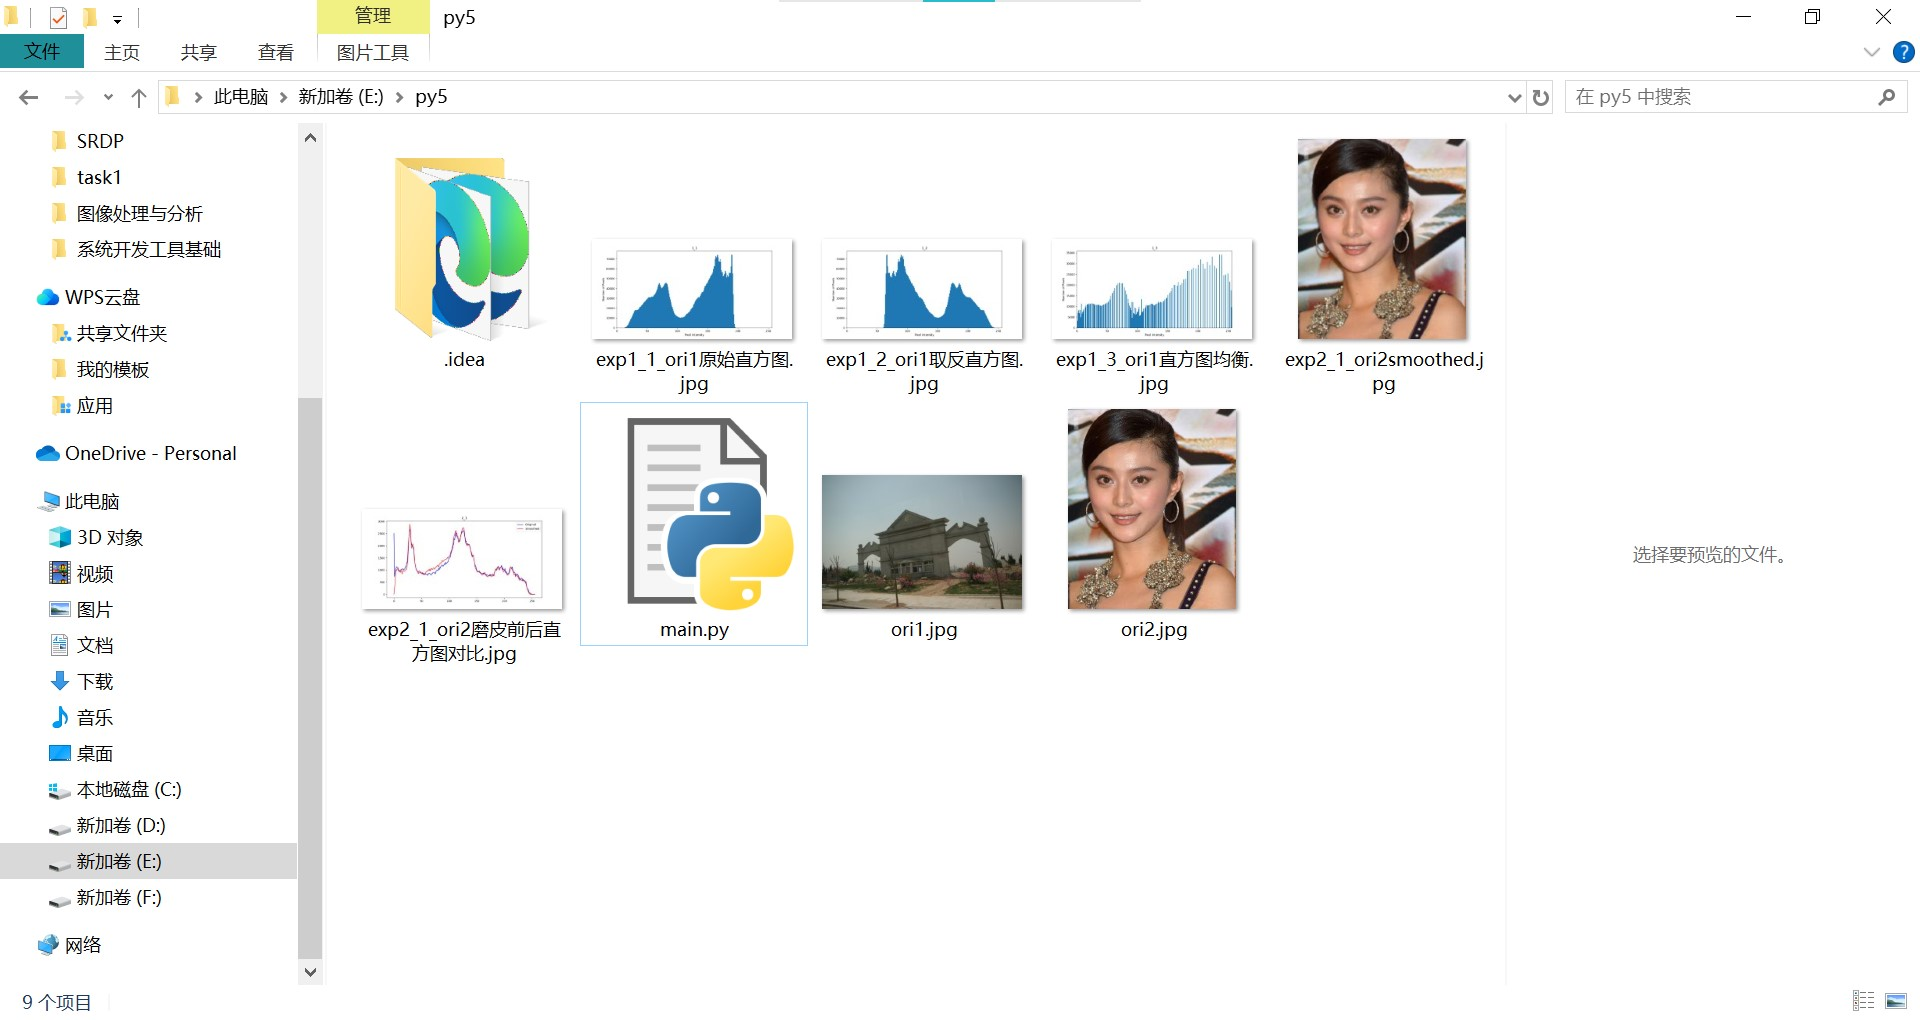
\includegraphics[width=1\textwidth]{038.jpg}
	\end{figure}
	
	\paragraph{(20)python视觉-油滴检测:}
	在pycharm写Python程序检测图片中的油滴并进行填色处理,保存结果。
	
	\paragraph{实例要求:}
	图片为海水中漏油溢出的油滴;请标记出图片中清晰的油滴并对其进行填色处理。
	
	\paragraph{实例解答:}
	分为如下五步:
	
	(1)设置图像列表。
	
	(2)通过灰度值区分检测油滴轮廓。具体思路是:cv2.imread()读取图像,对列表中的每个图像,cv2.cvtColor()转换为灰度图像;应用高斯模糊cv2.GaussianBlur()减少噪声;cv2.inRange()创建掩膜覆盖灰度值为0到95的区域,即油滴区域(这里也可通过二值化操作,将阈值设为95区分油滴区域);进行形态学开运算操作,即即先腐蚀(cv2.erode()函数),再对腐蚀结果进行膨胀(cv2.dilate()函数),目的是去噪、便于提取轮廓;对处理后的掩膜提取轮廓,即得到油滴轮廓。

	(3)对每个提取到的轮廓,cv2.drawContours()进行填色处理。
	
	(4)用plt库函数将处理后的照片与原图并列展示,以体现填色效果。根据填色效果适当手动调节掩膜的灰度范围以达到更好的效果。
	
	(5)保存填色后的图像。
	
	(具体代码及输出结果已上传至github库-task2-py6)
	
	\begin{figure}[H]
		\centering
		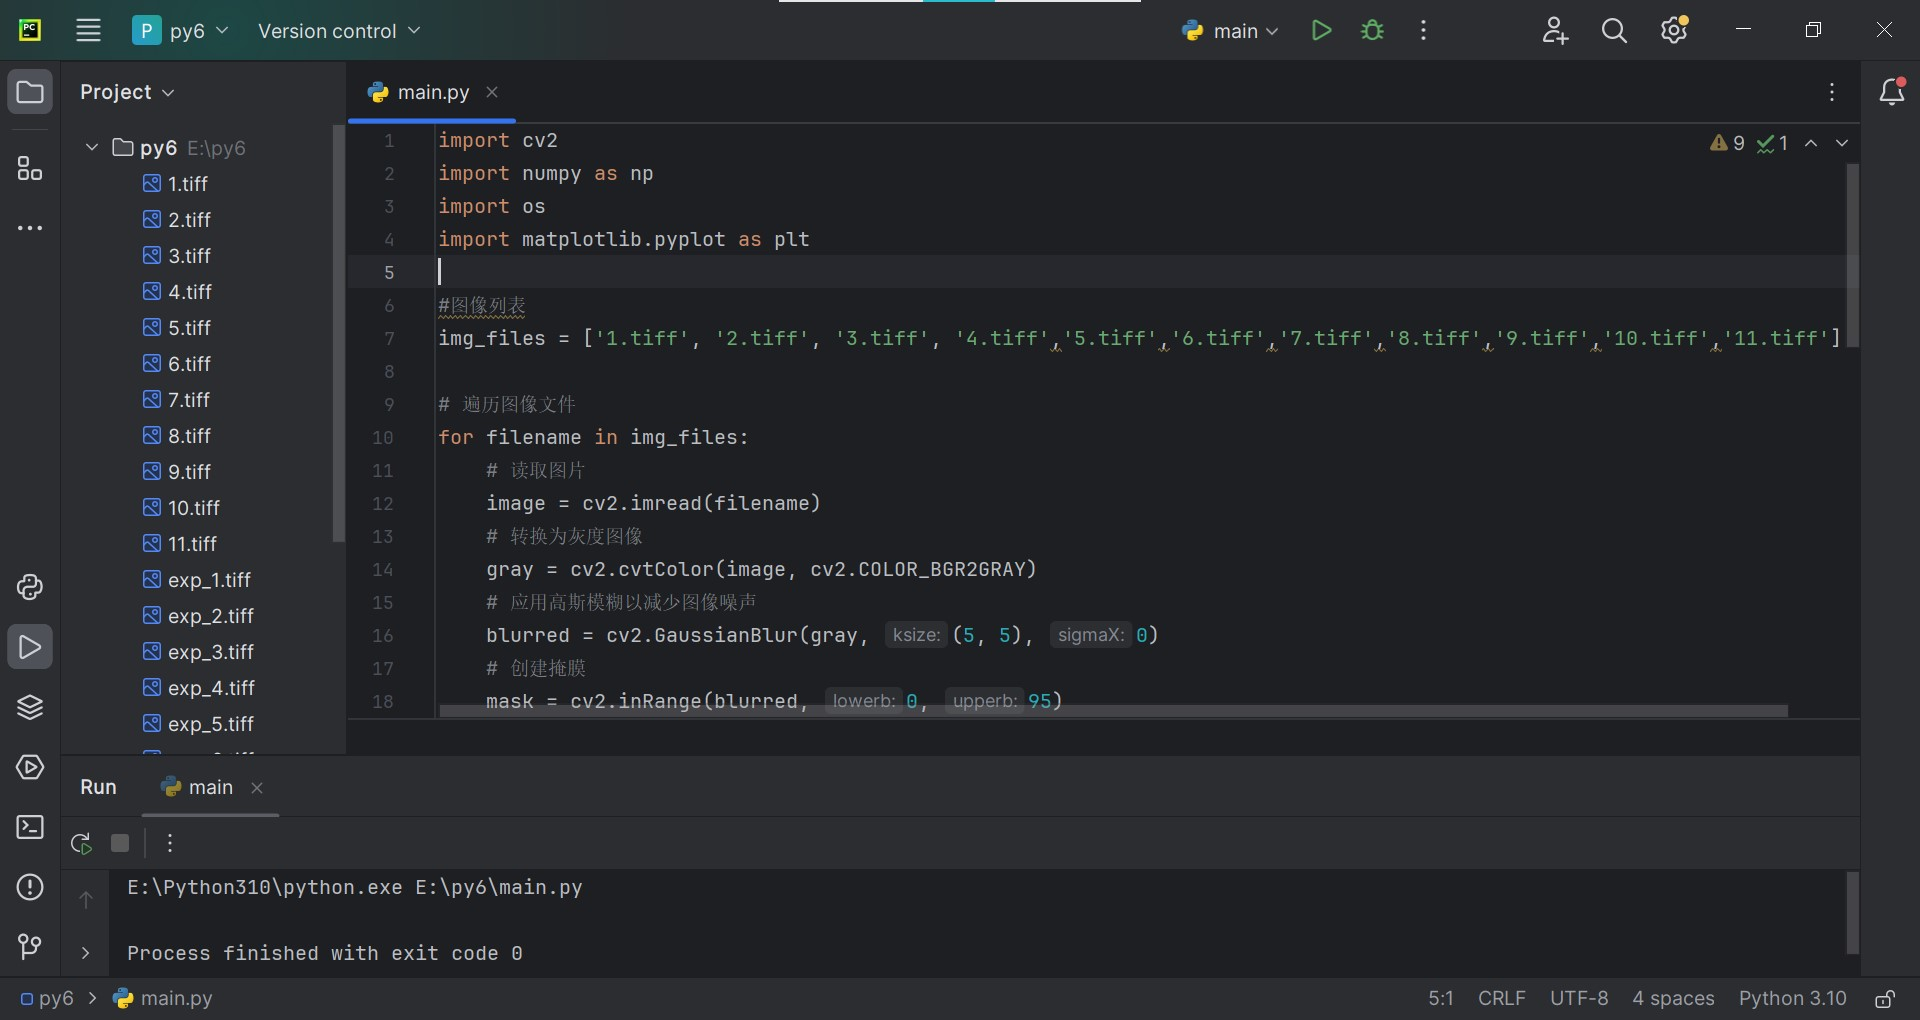
\includegraphics[width=1\textwidth]{039.jpg}
		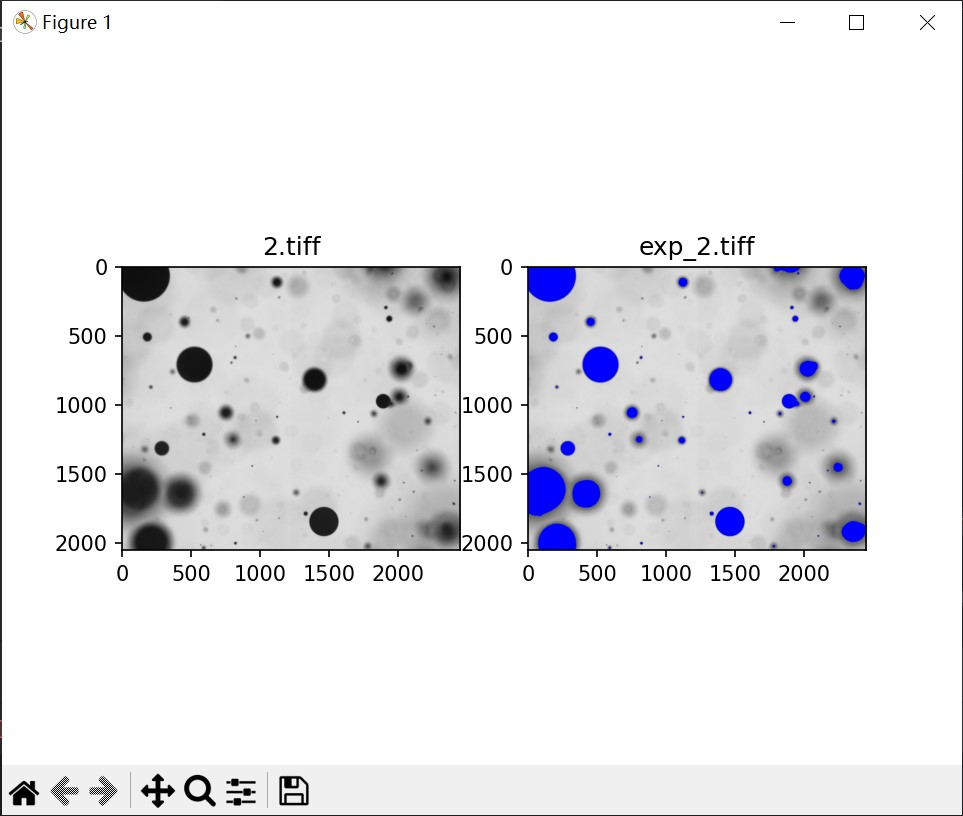
\includegraphics[width=1\textwidth]{040.jpg}
		
\includegraphics[width=1\textwidth]{041.jpg}
	\end{figure}
	
	\section{问题及解决方案}
	
	\paragraph{(1)}
	问题:安装tmux时报错。
	
	解决方案:这台虚拟机的网络环境有问题,换了一台虚拟机后成功安装。
	
	\begin{figure}[h]
		\centering
		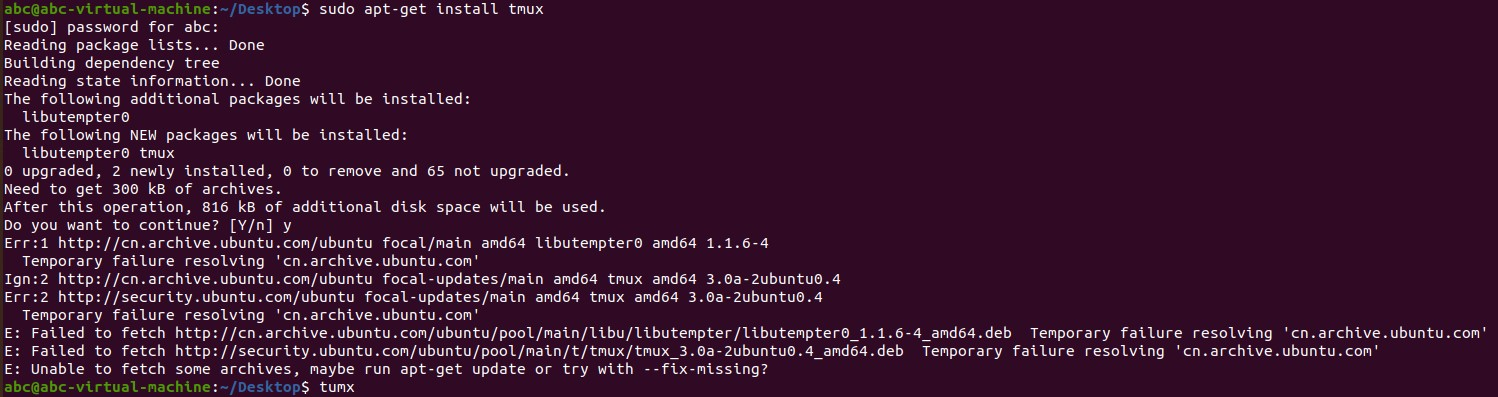
\includegraphics[width=1\textwidth]{009.jpg}
		
\includegraphics[width=1\textwidth]{011.jpg}
	\end{figure}
	
	\section{解题感悟}
	这次实验内容包括命令行环境、Python入门基础和Python视觉应用。通过本实验我掌握了tmux、修改配置、管理进程、编写python程序、引用cv库和plt库等库的库函数进行图像处理等技能。
	
	通过练习命令行部分的习题,我掌握了使用pgrep和pkill等命令来高效管理进程、使用tmux进行终端多路复用以同时执行多个任务、创建别名代替一长串包含许多选项的命令以提高效率。通过学习这部分内容的知识,我对命令行环境的高效使用有了更深入的理解。
	
	在Python入门基础和Python视觉应用方面,由于我上学期修了图像处理与分析,练习了足够多了python题目,所以较为熟练。python有着丰富的库,与其他编程语言相比,python在视觉图像处理方面有着无可比拟的优势。在本实验中我温习了Python的基本语法和Python在图像处理领域的应用,进一步锻炼了编程能力。
	
	\section{github链接}
	\underline{https://github.com/zxm2580/xtkfgjjc-202408.git}	
	
\end{document}